%%%%%%%% ICML 2026 EXAMPLE LATEX SUBMISSION FILE %%%%%%%%%%%%%%%%%

\documentclass{article}

% Recommended, but optional, packages for figures and better typesetting:
\usepackage{microtype}
\usepackage{graphicx}
\usepackage{subfigure}
\usepackage{booktabs} % for professional tables
\usepackage{array}
\usepackage{comment}
\usepackage{placeins}
% hyperref makes hyperlinks in the resulting PDF.
% If your build breaks (sometimes temporarily if a hyperlink spans a page)
% please comment out the following usepackage line and replace
% \usepackage{icml2026} with \usepackage[nohyperref]{icml2026} above.
\usepackage{hyperref}


% Attempt to make hyperref and algorithmic work together better:
\newcommand{\theHalgorithm}{\arabic{algorithm}}

% Use the accepted option for the camera-ready version.
\usepackage[accepted]{icml2026}

% For preprint, use
% \usepackage[preprint]{icml2026}

% If accepted, instead use the following line for the camera-ready submission:
% \usepackage[accepted]{icml2026}

\usepackage{amsmath}
\usepackage{amssymb}
\usepackage{mathtools}
\usepackage{amsthm}

\DeclareMathOperator{\ReLU}{ReLU}
\newcommand{\relu}{\ensuremath{\ReLU}}

\newcolumntype{L}[1]{>{\raggedright\arraybackslash}p{#1}}


% if you use cleveref..
\usepackage[capitalize,noabbrev]{cleveref}

%%%%%%%%%%%%%%%%%%%%%%%%%%%%%%%%
% THEOREMS
%%%%%%%%%%%%%%%%%%%%%%%%%%%%%%%%
\theoremstyle{plain}
\newtheorem{theorem}{Theorem}[section]
\newtheorem{proposition}[theorem]{Proposition}
\newtheorem{lemma}[theorem]{Lemma}
\newtheorem{corollary}[theorem]{Corollary}
\theoremstyle{definition}
\newtheorem{definition}[theorem]{Definition}
\newtheorem{assumption}[theorem]{Assumption}
\theoremstyle{remark}
\newtheorem{remark}[theorem]{Remark}

% Todonotes is useful during development; simply uncomment the next line
%    and comment out the line below the next line to turn off comments
\usepackage[disable,textsize=tiny]{todonotes}
%\usepackage[textsize=tiny]{todonotes}

% The \icmltitle you define below is probably too long as a header.
% Therefore, a short form for the running title is supplied here:
\icmltitlerunning{Dropout Universality: Scaling Laws and Optimal Scheduling at the Edge-of-Chaos}

\begin{document}

\twocolumn[
  \icmltitle{Dropout Universality: Scaling Laws and Optimal Scheduling at the Edge-of-Chaos}

  % It is OKAY to include author information, even for blind submissions: the
  % style file will automatically remove it for you unless you've provided
  % the [accepted] option to the icml2026 package.

  % List of affiliations: The first argument should be a (short) identifier you
  % will use later to specify author affiliations Academic affiliations
  % should list Department, University, City, Region, Country Industry
  % affiliations should list Company, City, Region, Country

  % You can specify symbols, otherwise they are numbered in order. Ideally, you
  % should not use this facility. Affiliations will be numbered in order of
  % appearance and this is the preferred way.
  \icmlsetsymbol{equal}{*}

  \begin{icmlauthorlist}
    \icmlauthor{Lucas Fernandez Sarmiento}{cmu}
  \end{icmlauthorlist}

  \icmlaffiliation{cmu}{Carnegie Mellon University (CMU), Pittsburgh, Pennsylvania, USA}

  \icmlcorrespondingauthor{Lucas Fernandez Sarmiento}{lucasf@andrew.cmu.edu}

  % You may provide any keywords that you find helpful for describing your
  % paper; these are used to populate the "keywords" metadata in the PDF but
  % will not be shown in the document
  \icmlkeywords{Machine Learning, ICML}

  \vskip 0.3in
]

% this must go after the closing bracket ] following \twocolumn[ ...

% This command actually creates the footnote in the first column listing the
% affiliations and the copyright notice. The command takes one argument, which
% is text to display at the start of the footnote. The \icmlEqualContribution
% command is standard text for equal contribution. Remove it (just {}) if you
% do not need this facility.

% Use ONE of the following lines. DO NOT remove the command.
% If you have no special notice, KEEP empty braces:
\printAffiliationsAndNotice{}  % no special notice (required even if empty)
% Or, if applicable, use the standard equal contribution text:
% \printAffiliationsAndNotice{\icmlEqualContribution}

\begin{abstract}
We develop a mean-field theory of dropout as a perturbation of critical signal propagation at the edge of chaos. Dropout shifts the perfect-alignment fixed point, making the depth scale for information propagation finite even at critical initialization. We derive critical and crossover scaling laws for correlation decay and establish that smooth activations and kinked, \relu{}-like activations constitute distinct universality classes, with different critical exponents and a universal two-parameter scaling collapse in detuning and dropout strength. The distinction traces to the analytic structure of the correlation map: smooth activations admit a Taylor expansion near perfect alignment, while kinked activations develop a branch point with universal non-analyticity. As a corollary, the framework yields principled dropout schedules that maximize effective correlation length under fixed budget, giving higher held-out test accuracy and lower held-out test loss at no extra computational cost. We test the predictions in MLPs and Vision Transformers and discuss CNN/ResNet extensions.
\end{abstract}










\section{Introduction}

Mean-field analyses of randomly initialized deep networks reveal an order-to-chaos phase diagram that controls both signal propagation and gradient penetration with depth \cite{poole2016exponentialexpressivitydeepneural,schoenholz2017deepinformationpropagation,Bahri2020StatMechDeepLearning,bahri2024leshoucheslecturesdeep}. In this work, we give a holistic exploration of how this picture is modified by dropout. Using the representation-group (coarse-graining) language of \cite{roberts2022principlesdeeplearningtheory,bahri2024leshoucheslecturesdeep}, we show that dropout behaves as a relevant perturbation: it displaces the critical fixed point and grows under depth coarse-graining, pushing the dynamics away from criticality and determining the macroscopic phase. Concretely, dropout deforms the correlation map \cite{schoenholz2017deepinformationpropagation} by adding a correlation-independent shift at perfect alignment, so that perfect correlation between inputs is no longer a fixed point for any nonzero dropout. Thus, even at the edge-of-chaos \cite{sompolinsky1988chaos,packard1988adaptation,bertschinger2004real}, the depth correlation length is finite. We interpret this shift as an equation of state for the decorrelation order parameter $m \equiv 1-c^\ast$ (with $c^\ast$ the asymptotic inter-signal correlation), derive the resulting scaling laws, and show that smooth and kinked, \relu{}-like activations exhibit the same qualitative phase diagram but different critical scaling in the presence of dropout.

Additionally, we show that the two control parameters (dropout strength and distance to criticality) admit a scaling collapse into a single universal form,\footnote{This is analogous to the homogeneous scaling of connected correlation functions near a critical point; related scaling forms hold for one-particle-irreducible vertex functions after the usual Legendre transform \cite{ZinnJustin2002QFTCritical}.} and we illustrate how these predictions compare with mean-field recursions. 

This analysis yields three main conceptual contributions. First, while dropout was previously shown to destroy the order-to-chaos critical point \cite{schoenholz2017deepinformationpropagation}, we show that the deformed mean-field map still retains a nontrivial $c^\ast<1$ fixed point. This keeps the correlation length recursion and yields a Landau equation of state for $m=1-c^\ast$ together with a two-parameter scaling collapse. Second, we show that universality classes and scaling laws are set by activation smoothness: smooth and kinked activations have distinct critical exponents (Table~\ref{tab:critical_exponents}), a distinction reflected in their Hermite spectral structure (App.~\ref{sec:var-opt-act}). Since the same Gaussian activation kernels arise beyond MLPs, including CNNs and residual branches (App.~\ref{app:cnn_extension}), we expect the qualitative smooth/kinked split to be a well-motivated heuristic. Third, we treat dropout as a depth-dependent dynamical field, and optimizing the effective correlation length functional with respect to this field yields first-principles dropout schedules that we validate experimentally at fixed budget. Treating classically fixed hyperparameters as fields that can change through the network opens a new dimension for hyperparameter optimization across depth, and potentially over training time. If the reader takes away only one thing from this paper, we hope it is the three ideas outlined above.

This work complements prior studies of depth-dependent regularization: stochastic depth drops whole residual blocks with increasing probability \cite{huang2016deep}, curriculum dropout anneals dropout over training time \cite{morerio2017curriculum}, and LayerDrop removes transformer layers for efficiency \cite{fan2019reducing}. Our schedules are spatial depth profiles, so they are complementary to temporal curricula and layer-dropping mechanisms. Qualitatively different edge-of-chaos behavior for smooth and \relu{}-like activations was previously observed in \cite{hayou2019impact}; here we extract the scaling exponents and identify the corresponding universality classes.










\section{Mean-field theory background}
\label{sec:mft_background}
We first state the mean-field assumptions for MLPs, which provide the baseline for the dropout analysis \cite{poole2016exponentialexpressivitydeepneural,schoenholz2017deepinformationpropagation,Bahri2020StatMechDeepLearning,bahri2024leshoucheslecturesdeep}. We consider fully-connected MLPs at random initialization, where preactivations are well-approximated as Gaussian random variables with self-consistently determined statistics (means, variances, covariances). In the strict infinite width limit this Gaussian description becomes exact \cite{Lee2018DNNasGP}, while at large but finite width deviations from Gaussianity can be organized perturbatively in the depth-to-width aspect ratio (schematically $L/N$), as treated comprehensively in \cite{roberts2022principlesdeeplearningtheory,bahri2024leshoucheslecturesdeep}. The intuition behind this treatment is that as we add more activations, through the CLT, the statistics will become more and more Gaussian, approaching this distribution asymptotically in the large N limit. 

We consider an MLP of depth $L$, $N_l$ neurons in layer $l$, and an activation $\phi:\mathbb{R}\to\mathbb{R}$ (e.g.\ $\tanh$, \relu{}, \emph{etc.}). We use the standard i.i.d.\ Gaussian initialization
%
\begin{equation}
W^{l}_{ij}\sim \mathcal{N}\!\left(0,\frac{\sigma_{w}^{2}}{N_{l}}\right), \qquad b^{l}_{i}\sim \mathcal{N}\!\left(0,\sigma_{b}^{2}\right),
\end{equation}
%
take the input as $y^{0}_{i;a}=x_{i;a}$, and propagate forward via
%
\begin{equation}
z^{\,l}_{i;a}= W^{l}_{ij}\,y^{\,l}_{j;a}+b^{l}_{i}, \qquad y^{\,l+1}_{i;a}=\phi\!\left(z^{\,l}_{i;a}\right),
\end{equation}
%
where $a$ labels the input. Throughout, expectations $\mathbb{E}[\cdot]$ are over the random weights and biases at initialization, with inputs held fixed. We also use the standard Gaussian measure
%
\begin{equation}
\int Dz\,(\cdots)\;\equiv\;\frac{1}{\sqrt{2\pi}}\int_{-\infty}^{\infty}dz\,e^{-z^{2}/2}(\cdots),
\end{equation}
%
and similarly for $\int Dz_1 Dz_2$.

In the infinite-width limit this becomes exact layer-by-layer, while at finite width the first layer is exactly Gaussian (being a linear map of fixed inputs) and subsequent layers are only approximately Gaussian, with controlled non-Gaussian corrections parametrized by the depth-to-width ratio \cite{roberts2022principlesdeeplearningtheory}. A fuller treatment of the MFT background is given in App.~\ref{app:mft_primer}. 

We track the single-input preactivation variance $q^l_{aa}$, the two-input covariance $q^l_{ab}$, and the induced correlation $c^l_{ab}$:
%
\begin{align}
q^{\,l}_{aa}&= \sigma_{w}^{2}\int Dz\,\phi^{2}\!\left(\sqrt{q^{\,l-1}_{aa}}\,z\right)+\sigma_{b}^{2}\\
q^{\,l}_{ab}&=\sigma_{w}^{2}\int Dz_{1}\,Dz_{2}\,\phi(u_{1})\,\phi(u_{2})+\sigma_{b}^{2}\\
u_{1}&=\sqrt{q^{\,l-1}_{aa}}\,z_{1},\qquad c^{\,l-1}_{ab}=\frac{q^{\,l-1}_{ab}}{\sqrt{q^{\,l-1}_{aa}\,q^{\,l-1}_{bb}}},\\
u_{2}&=\sqrt{q^{\,l-1}_{bb}}\left(c^{\,l-1}_{ab} z_{1}+\sqrt{1-\left(c^{\,l-1}_{ab}\right)^{2}}\,z_{2}\right).
\label{variancerecursion}
\end{align}
%
In the absence of dropout, for a wide array of activations $q^{\,l}_{ab},c^{\,l}_{ab}$ settle to fixed points $q^*,c^*$; in particular, there exists a $c^*=1$ fixed point as a straightforward calculation shows. The variance fixed point sets the typical activation scale, while the correlation fixed point describes whether distinct inputs become indistinguishable under depth iteration. We denote the recurrence relation for $c^{\,l}_{ab}$ by $c^{\,l}_{ab}=F(c^{\,l-1}_{ab})$. 

To probe its stability, one linearizes the map at $c=1$, defining the (angular) susceptibility
%
\begin{equation}
\chi_{\perp} \equiv \left.\frac{\partial c^{\,l}_{ab}}{\partial c^{\,l-1}_{ab}}\right|_{c_{ab}=1} = \sigma_{w}^{2}\int Dz \,\big[\phi'(\sqrt{q^{*}}\,z)\big]^{2}.
\end{equation}
%
This creates a phase diagram with three regimes: $\chi_{\perp}<1$ is the ordered regime, $\chi_{\perp}>1$ is chaotic, and 
 $\chi_{\perp}=1$ defines the critical regime (the so-called "edge-of-chaos"). The depth scale controlling cross-input correlations can become arbitrarily large in the latter, allowing information to penetrate deep into the network. For \relu{}, the criticality condition gives $\sigma_w^2=2$, coinciding with the variance used in He initialization \cite{he2015delvingdeeprectifierssurpassing}\footnote{This is not true for general activations, but rather an idiosyncrasy of \relu{}} (see App.~\ref{app:mft_primer}), a more fundamental viewpoint than variance preservation. 
 
 This leads to an emergent characteristic depth scale $\xi_c$, which parametrizes both signal propagation and gradient flow. Iterating random affine maps induces an effective coarse-graining in depth akin to renormalization-group flow, called representation group flow in the ML context \cite{roberts2022principlesdeeplearningtheory}; information about norms and angles relaxes exponentially fast,
%
\begin{equation}
|{c^*-c^l_{ab}}|\propto e^{-l/\xi_{c}}, \qquad \xi_{c}^{-1}\equiv -\log|r_{c}|.
\label{corrq}
\end{equation}
%
An analogous correlation length $\xi_q$ controls how quickly single-input norms settle to $q^{*}$. Heuristically, $\xi_{c}$ controls how far distinctions between different inputs survive with depth; in the ordered phase $c^{*}=1$, so $u_{1}^{*}=u_{2}^{*}$ and $\xi_{c}^{-1}=-\log\chi_{\perp}$, hence $\chi_{\perp}\to 1$ implies $\xi_{c}\to\infty$. Consequently, the edge-of-chaos is primarily about $\xi_{c}$ rather than $\xi_{q}$, except in special cases. For \relu{}, the curvature vanishes everywhere away from the origin, leading to a coincidence between $\xi_c$ and $\xi_q$, both diverging as $\chi_{\perp}\to 1$, provided a finite $q^{*}$ exists. This is one concrete reason why \relu{}-style near-critical initializations are comparatively forgiving in practice.

As previously discussed, mean-field theory is an expansion in non-Gaussian corrections suppressed by powers of \(L/N\). Therefore, in our experiments we work in a controlled regime with \(L/N \ll 1\) (i.e., \(N \gg L\)), where the large-width expansion is controlled \cite{roberts2022principlesdeeplearningtheory}. The correlation length diverges as we approach criticality, amplifying finite-width and other non-Gaussian corrections. Thus, when probing critical power laws with dropout, we keep the dropout rate small but non-negligible: infinitesimal dropout would require prohibitively deep networks to estimate the correlation length and related quantities.

Although we derive these results for MLPs, analogous large-width limits exist elsewhere. CNNs are the canonical convolutional setting \cite{cnnslecun}, and at infinite channel count their covariance recursions again close through Gaussian activation kernels \cite{xiao2018dynamicalisometrymeanfield}. ResNets are especially suggestive: Yang and Schoenholz \cite{yang2017meanfieldresnets} find qualitatively different tanh/\relu{} large-depth behavior. Skip connections alter global depth dynamics, easing the information propagation by injecting the original signal after every layer, changing exponential convergence to subexponential or polynomial laws and allowing norm drift, but each residual branch still inherits the local nonlinear Gaussian kernel. Thus our smooth/kinked universality split offers a possible theoretical explanation for their observed dichotomy; a dropout-deformed ResNet theory is left for future work. For transformers \cite{vaswani2023attentionneed}, related infinite-width attention analyses use large hidden dimension and/or many heads \cite{Hron2020InfiniteAttention}. Because the exponents are controlled by the local analytic structure of this channel, we expect the mechanism to persist when it controls the wide-limit recursion. In Sec.~\ref{subsec:optimal_dropout}, we test this extrapolation in transformers.

In App.~\ref{app:experimental_info} we probe realistic scenarios across architectures, datasets, and schedules. We focus on overparameterized regimes where dropout improves generalization and accuracy, and thus where it is used in practice, and we explicitly study the trade-off between dropout-driven regularization and stable signal propagation. The mean-field objective predicts sparse, step-like allocation at fixed budget, but it is permutation invariant in depth and therefore cannot by itself decide where dropout should be concentrated. To break this degeneracy we appeal to effects outside the mean-field closure, such as early coadaptation and rank collapse: these make the first layers the most valuable place to inject noise, explaining why front-loaded schedules work best in the experiments.










\section{Universality Classes and Critical Scaling under Dropout}


Dropout \cite{srivastava2014dropout,wager2013dropout} is often used as a regularizer that reduces overfitting by randomly masking activations during training, thereby reducing the network’s reliance on any single subset of pathways and discouraging co-adaptation. In the previous literature, dropout was explored in MFT \cite{lee2019mean, schoenholz2017deepinformationpropagation}, but not in the universality class sense. We formalize dropout as multiplicative Bernoulli noise applied post-activation,
%
\begin{equation}
p^{(\ell)}_{j} \sim \mathrm{Bernoulli}(\rho), \qquad y^{(\ell)}_j \;\mapsto\; \tilde y^{(\ell)}_j \equiv \frac{p^{(\ell)}_{j}}{\rho}\,y^{(\ell)}_j,
\end{equation}
%
i.e.\ the standard inverted-dropout convention in which $\mathbb E_p[\tilde y^{(\ell)}_j]=y^{(\ell)}_j$, and hence $\mathbb E_p[\tilde z^\ell_i\mid W,b]=z^\ell_i$, so the mean preactivation is invariant to the dropout rate \cite{schoenholz2017deepinformationpropagation}. Throughout, $\rho$ is the keep probability. When comparing two inputs, we draw the dropout masks independently for each input\footnote{Correlated dropout masks can alleviate this detuning: if the same mask is shared across the batch, the \(c=1\) fixed point is preserved and near-critical scaling can be recovered by retuning, but the noise becomes batch coupled and the regularization is correspondingly weaker and more structured. We leave detailed analysis of correlated masks to future work.}; this independence is the source of the decorrelation effect analyzed below.

This distinction originally emerged from the following variational question: among activations of fixed scale, which functions make the correlation length of the near-critical Gaussian channel as large as possible? Extremizing the correlation length functional shows that the natural eigenfunctions of this problem are Hermite polynomials. When standard nonlinearities are decomposed in that basis, two qualitatively different spectra emerge. Smooth, analytic activations such as $\tanh$ have exponentially decaying Hermite coefficients, so their effect is dominated by the first few modes. Kinked activations such as \relu{} have power-law tails instead: the kink keeps exciting higher Hermite modes, leaving a broader spectrum in the correlation map. This spectral split was the original diagnostic for the smooth/kinked universality classes, which later reappears in the dropout scaling laws. The details of these computations can be found in App.~\ref{sec:var-opt-act}.

Our classification is orthogonal to the scale-invariant vs. non-scale-invariant distinction of \cite{roberts2022principlesdeeplearningtheory}: the multi-scale Hermite spectrum highlighted above is controlled primarily by analytic regularity (kinks and other non-analytic structure), not by scale invariance per se. The criterion is based on two facts: (a) near-critical scaling laws differ between smooth and kinked activations, and (b) the Hermite spectral weight of non-analytic activations decays as a power law, in contrast to the exponential decay characteristic of smooth activations (Apps.~\ref{ap:exponent_derivations} and~\ref{sec:var-opt-act}).

It is in this context that we seek a sharper analytical understanding of how dropout deforms the edge-of-chaos. Extending mean-field propagation to include dropout, one finds that for a single input dropout largely acts as a renormalization of the effective weight variance, $\sigma_w^2\mapsto \sigma_w^2/\rho$, but for two inputs the perfect-alignment fixed point at $c^*=1$ is lost for any $\rho<1$ when the two dropout masks are chosen independently \cite{schoenholz2017deepinformationpropagation}. In other words, dropout acts as an explicit symmetry-breaking ``field'' for alignment: even if two inputs are perfectly aligned at some depth, the next layer produces $\bar c_{ab}<1$, cutting off the divergence of the depth correlation length at the edge.

Introducing multiplicative Bernoulli noise with keep probability $\rho$, the perturbed preactivations read
%
\begin{equation}
z_i^\ell = \frac{1}{\rho} \sum_j W_{ij}^\ell \,p_j^\ell \,y_j^\ell + b_i^\ell.
\end{equation}
%
The single-input variance recursion becomes
%
\begin{equation}
\bar{q}_{aa}^{\,\ell} = \frac{\sigma_{w}^{2}}{\rho} \int \! Dz\, \phi^{2}\!\left( \sqrt{\bar{q}_{aa}^{\,\ell-1}}\, z \right) + \sigma_{b}^{2},
\end{equation}
%
where the bar reminds us that the variance fixed point is shifted by dropout. We denote the (putative) dropout variance fixed point by
%
\begin{equation}
\bar q^{*} \;=\; \frac{\sigma_w^2}{\rho}\int Dz\,\phi^2\!\big(\sqrt{\bar q^{*}}\,z\big) + \sigma_b^2.
\label{eq:qstar-dropout}
\end{equation}
%
For two distinct inputs $a\neq b$, we find a dropout shift at perfect alignment. If at some depth $c^{\ell}_{ab}=1$, then at the next layer one finds \cite{schoenholz2017deepinformationpropagation}
%
\begin{equation}
\bar F_\rho(1)= \bar c^{\,\ell+1}_{ab} = 1 - \frac{1 - \rho}{\rho \bar{q}^{*}} \sigma_{w}^{2} \int \! Dz\, \phi^{2}\!\left( \sqrt{\bar{q}^{*}}\, z \right).
\end{equation}
%
It is therefore natural to define the dropout field
%
\begin{align}
h &\;\equiv\; 1-\bar F_\rho(1)\nonumber\\
&\;=\; \frac{1-\rho}{\rho \bar q^{*}}\; \sigma_w^2\!\int Dz\,\phi^2\!\big(\sqrt{\bar q^{*}}\,z\big).
\label{eq:Delta_exact}
\end{align}
%
By construction, $
\rho<1
\Rightarrow
h>0,$
so the fixed point at $c^*=1$ is immediately spoiled: even if two inputs are perfectly aligned at some depth, the next layer produces $\bar c_{ab}=1-h<1$. Since we focus on weak dropout, it is useful to perform the small-\(\delta\rho\) expansion. Writing $\delta\rho\equiv 1-\rho$ with $\delta\rho\ll 1$, we have
$\bar q^*=q^*+\mathcal O(\delta\rho)$, so to leading order we have
%
\begin{equation}
h = \delta\rho\; \frac{\sigma_w^2}{\bar q^{*}}\!\int Dz\,\phi^2\!\big(\sqrt{\bar q^{*}}\,z\big) + \mathcal O(\delta\rho^2).
\label{eq:Delta_weakdrop}
\end{equation}
%
The backward pass has the same source of asymmetry. Let \(\delta^\ell_{j,a}\) be the backpropagated preactivation gradient for input \(a\). With inverted dropout,
%
\begin{equation}
\delta^\ell_{j,a} = \frac{p^\ell_{j,a}}{\rho}\, \phi'(u^\ell_{j,a}) \sum_i W^{\ell+1}_{ij}\delta^{\ell+1}_{i,a},
\end{equation}
%
up to convention-dependent layer indexing. If \(G^\ell_{ab}\equiv \mathbb E[\delta^\ell_a\delta^\ell_b]\) denotes the two-input gradient covariance, the wide-limit recursion contains
%
\begin{equation}
G^\ell_{ab} = \sigma_w^2 \mathbb E\!\left[ \frac{p^\ell_a p^\ell_b}{\rho^2} \phi'(u_a)\phi'(u_b) \right] G^{\ell+1}_{ab}.
\end{equation}
%
Thus independent masks give a diagonal factor \(\mathbb E[p_a^2]/\rho^2=1/\rho\) but an off-diagonal factor \(\mathbb E[p_a p_b]/\rho^2=1\). Dropout inflates single-sample gradient variance without similarly inflating cross-sample covariance, mirroring the forward asymmetry that produced \(h\). After normalization this suggests a backward field \(h_\nabla(\rho)\) that moves perfect gradient alignment below one. We do not identify it with the forward field: the backward kernel is built from \(\phi'\), not \(\phi\), and for \relu{} \(\phi'\) is discontinuous. A full dropout-deformed backward critical theory, including finite-width gradient susceptibilities and training-time mask correlations, is left for future work.










\subsection{Landau theory and critical exponents}

For smooth activations, the dropout-deformed correlation edge admits a simple Landau-style description in terms of
three mean-field variables:
%
\begin{equation}
m \equiv 1-c^*, \qquad t \equiv \chi_\rho-1, \qquad h \equiv 1-\bar F_\rho(1).
\end{equation}
%
The fields \((m,t,h)\) are chosen to mirror statistical-mechanics notation: \(t\) plays the role of a reduced temperature, \(m\) is the order parameter (magnetization), and \(h\) is an external field conjugate to \(m\) that explicitly biases the system away from perfect alignment.

We assume inverted dropout with keep probability \(\rho\in(0,1]\), with masks drawn i.i.d.\ across units and
independently across inputs. Let \(\bar q^*\) denote the dropout variance fixed point \eqref{eq:qstar-dropout}.
For an activation for which Price's theorem applies and \(\phi',\phi''\in L^2(\mathcal N(0,\bar q^\ast))\) (for instance, \(\phi\in C^2\) with sufficient Gaussian integrability) repeated application of Price's theorem gives the first two
derivatives of the correlation map at perfect alignment,\footnote{The \(\rho\)-dependence is implicit
through \(\bar q^*\). The full computation is given in App.~\ref{app:price_dropout}.}
%
\begin{align}
\chi_\rho &\equiv \bar F_\rho'(1) = \sigma_w^2\!\int Dz\,\big[\phi'(\sqrt{\bar q^{*}}\,z)\big]^2,
\label{eq:chi_dropout}\\
g_\rho &\equiv \bar F_\rho''(1) = \sigma_w^2\,\bar q^{*}\!\int Dz\,\big[\phi''(\sqrt{\bar q^{*}}\,z)\big]^2.
\label{eq:g_dropout}
\end{align}
%
In the smooth-class analysis below we assume \(g_\rho>0\). If \(g_\rho=0\), as for a linear activation, the quadratic Landau term is absent and the leading nonzero term determines a degenerate case rather than the generic smooth universality class.
For kinked, \relu{}-like activations, \(\bar F_\rho''(1)\) is not finite and the analytic expansion below is not the
correct organizing principle; we treat that universality class separately.

The Landau equation of state follows by expanding \(\bar F_\rho(c)\) around \(c=1\). Writing \(c^*=1-m\) with \(0<m\ll 1\) acting as the order parameter,
%
\begin{align}
\bar F_\rho(1-m)&=\bar F_\rho(1)-\chi_\rho m+\frac{g_\rho}{2}m^2+\mathcal O(m^3)\\
&=(1-h)-\chi_\rho m+\frac{g_\rho}{2}m^2+\mathcal O(m^3),
\end{align}
%
 imposing the fixed-point condition \(1-m=\bar F_\rho(1-m)\) yields
%
\begin{equation}
h + t\,m - \frac{g_\rho}{2}\,m^2 = 0, \quad\Longleftrightarrow\quad h = \frac{g_\rho}{2}\,m^2 - t\,m,
\label{eq:EoS_correct}
\end{equation}
%
with \(t\equiv \chi_\rho-1\). The physical (nonnegative) solution is
%
\begin{equation}
m(t,h) \;=\; \frac{t + \sqrt{t^2 + 2 g_\rho h}}{g_\rho}.
\label{eq:m_smooth_solution}
\end{equation}
%
At the correlation edge \(t=0\), dropout displaces the fixed point by
%
\begin{equation}
m(0,h) \;=\; \sqrt{\frac{2h}{g_\rho}}.
\label{eq:m_at_edge}
\end{equation}
%
\begin{table}[h]
\caption{Definitions of critical exponents in the thermodynamic limit ($t \to 0$, $h \to 0$).}
\label{tab:math_exponents}
\centering
\renewcommand{\arraystretch}{1.8}
\begin{tabular}{lc}
\toprule
Exponent & Mathematical Definition \\
\midrule
$\beta$ & $m \sim |t|^\beta \quad (h=0)$ \\
$\delta$ & $m \sim |h|^{1/\delta} \quad (t=0)$ \\
$\gamma$ & $\chi_M \equiv \left. \frac{\partial m}{\partial h} \right|_{h \to 0} \sim |t|^{-\gamma}$ \\
$\alpha$ & $C \equiv -\frac{\partial^2 f}{\partial t^2} \sim |t|^{-\alpha}$ \\
$\nu_t$ & $\xi \sim |t|^{-\nu_t} \quad (h=0)$ \\
$\nu_\rho$ & $\xi \sim |h|^{-\nu_\rho} \quad (t=0)$ \\
$\theta_{\rm rel}$ & $m \sim \ell^{-\theta_{\rm rel}} \quad (t=0,\, h=0)$ \\
\bottomrule
\end{tabular}
\end{table}

For the \(\alpha\) column we define the singular Landau potential \(f_{\rm sing}\) through the equation of state. In the smooth case,
%
\begin{equation}
\frac{\partial f_{\rm sing}}{\partial m} = -h-tm+\frac{g_\rho}{2}m^2,
\end{equation}
%
and in the kinked case,
%
\begin{equation}
\frac{\partial f_{\rm sing}}{\partial m} = -h-tm+\kappa m^{3/2}.
\end{equation}
%
Evaluating \(f_{\rm sing}\) on the stable branch at \(h=0\) gives \(f_{\rm sing}\sim |t|^3\) for the smooth class and \(f_{\rm sing}\sim |t|^5\) for the kinked class, hence \(\alpha=-1\) and \(\alpha=-3\), respectively.

This square-root power law is our first encounter with a larger family of critical exponents familiar in the physics literature, defined in Table~\ref{tab:math_exponents}. The key exponents for our analysis are those governing the depth correlation length $\xi_{c,\rho}$, as it sets the characteristic depth scale over which distinct inputs remain distinguishable and therefore provides an effective upper bound on the depth over which the network can reliably propagate information (and learn). Their derivations are straightforward but cumbersome, so we collect them in App.~\ref{ap:exponent_derivations} and simply quote the resulting exponent values in Table~\ref{tab:critical_exponents}. For reference, we also list the standard mean-field (Landau) exponents of the Ising universality class \cite{Ising1925,LandauLifshitzStatPhys} and the corresponding mean-field exponents of spin-glass theory \cite{EdwardsAnderson1975,Parisi1979PRL,Parisi1980JPA,Parisi1983PRL}. The SK entries are quoted in the standard mean-field convention and are meant as structural motivation--an order parameter without a simple \(\mathbb Z_2\) symmetry and a cubic effective interaction--not as a claim of shared universality: the smooth class shares the static entries \((\beta,\gamma,\delta,\alpha)\) in this convention, but not the correlation-length or relaxation exponents, while the kinked class is separated more sharply. The spin-glass comparison can be found in \cite{MezardParisiVirasoro1987,Parisi1983RMP,sherrington1975sk}.



\begin{table}[h]
\caption{Critical exponents for neural network initialization across different universality classes. The kinked \(\nu_\rho\) is a normal-form field exponent; ordinary bias-free \relu{} dropout follows the constrained path \(t=-h\) but has the same leading \(\xi\sim h^{-1/3}\) law (App.~\ref{ap:exponent_derivations}).}
\label{tab:critical_exponents}
\centering
\small
\setlength{\tabcolsep}{3pt}
\renewcommand{\arraystretch}{1.25}
\begin{tabular}{@{} l ccccccc @{}}
\toprule
\textbf{Universality Class} & $\boldsymbol{\nu_t}$ & $\boldsymbol{\beta}$ & $\boldsymbol{\theta}_{\rm rel}$ & $\boldsymbol{\gamma}$ & $\boldsymbol{\delta}$ & $\boldsymbol{\nu_\rho}$ & $\boldsymbol{\alpha}$ \\
\midrule
\textbf{Smooth activation}  & $1$ & $1$ & $1$ & $1$ & $2$ & $\frac{1}{2}$ & $-1$ \\[6pt]
\textbf{Kinked activation}  & $1$ & $2$ & $2$ & $1$ & $\frac{3}{2}$ & $\frac{1}{3}$ & $-3$ \\[6pt]
\textbf{Spin glass (SK MF)} & $\frac{1}{2}$ & $1$ & $2$ & $1$ & $2$ & $\frac{1}{4}$ & $-1$ \\[6pt]
\textbf{Ising-like}   & $\frac{1}{2}$ & $\frac{1}{2}$ & $1$ & $1$ & $3$ & $\frac{1}{3}$ & $0$ \\
\bottomrule
\end{tabular}
\end{table}

\vspace{0.25em}
\noindent
Figure~\ref{fig:dropout_scaling} summarizes these power laws from direct mean-field recursion and shows where higher-order corrections become visible away from the asymptotic regime.






\begin{figure*}[ht]
    \centering
    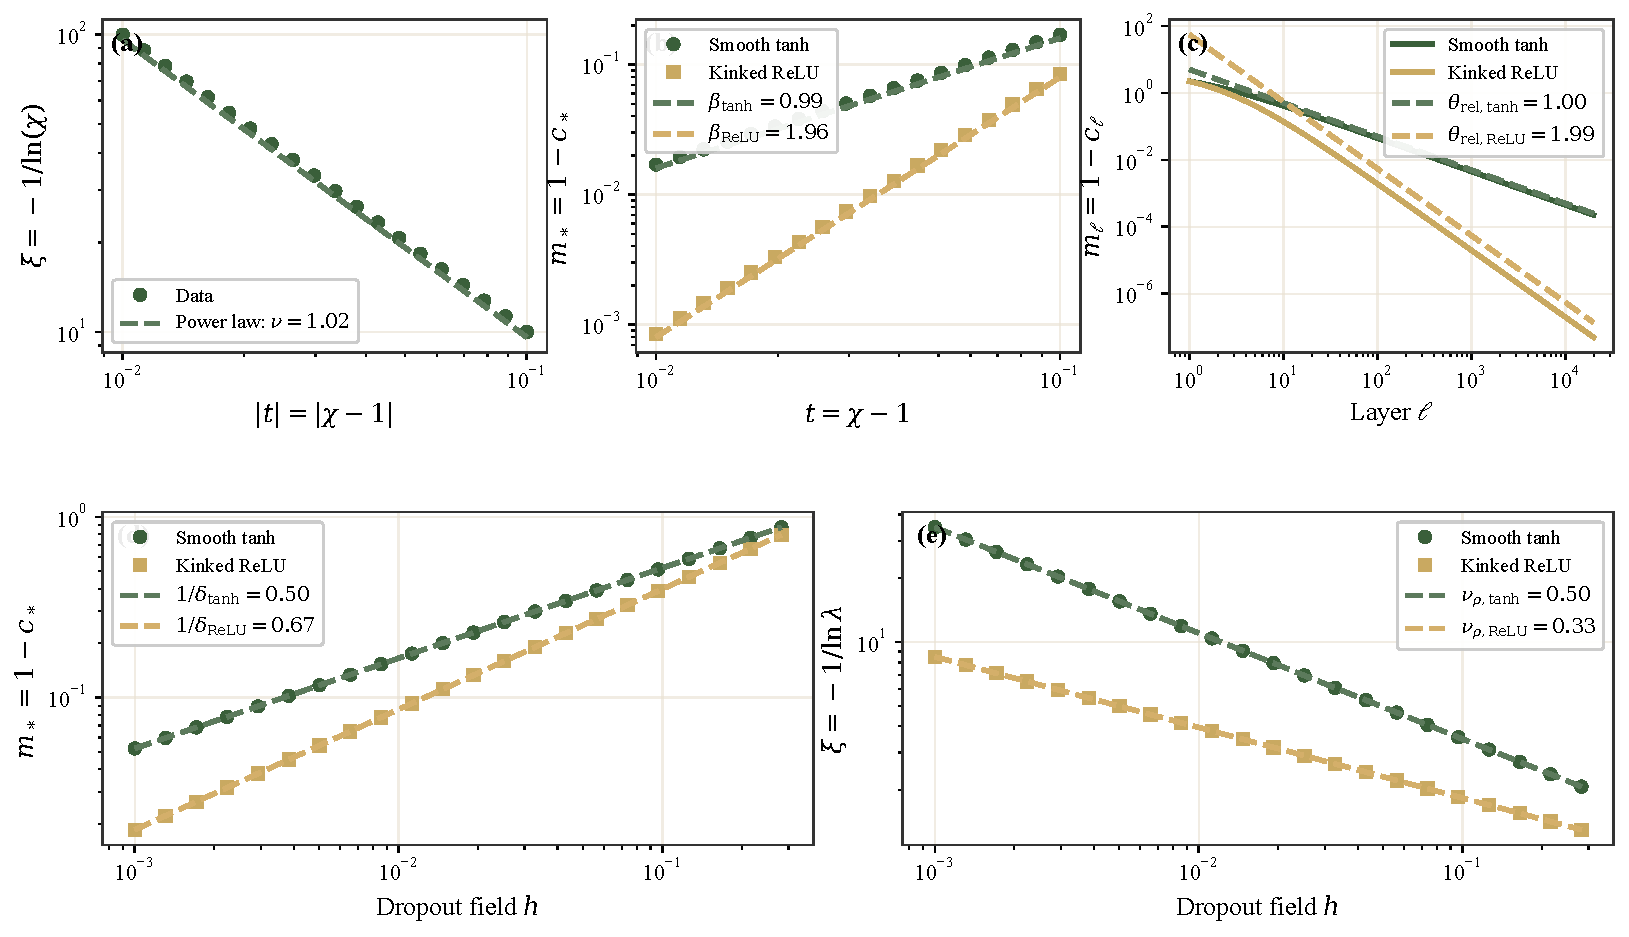
\includegraphics[width=1.0 \textwidth]{figures/theory/critical_exponents.pdf}
\caption{
Critical scaling for smooth (tanh) and kinked (\relu{}) activation functions, comparing tuning at zero dropout to tuning at the edge-of-chaos using a dropout field. The top row compares the different critical exponents at zero dropout and probes critical detuning decay, while the bottom row explores on critical networks with non-zero dropout. As the variables grow, higher-order effects become comparable and the linearized theory departs from the full recursion.}
    \label{fig:dropout_scaling}
\end{figure*}










\subsection{Scaling collapse and crossover region}
At leading normal-form order, dropout and detuning enter the same local equation of state. The collapse below is exact for the truncated Landau normal form, while the full mean-field recursion receives higher-order corrections such as \(\mathcal O(m^3)\) in the smooth case, \(\mathcal O(m^2)\) in the kinked case, and corrections from the nonlinear microscopic map \(h=\Delta(\rho)\). These corrections become visible away from the asymptotic near-critical regime. From the field-theory point of view, the resulting collapse is the standard signature of criticality: in the massless limit, connected \(n\)-point functions become homogeneous scaling functions of their separations, so the data collapse after rescaling by the appropriate critical dimensions \cite{ZinnJustin2002QFTCritical}.
In practice, experiments are rarely tuned exactly to the correlation edge \(t=0\) while simultaneously taking the dropout field to zero, \(h\to 0\). The useful near-critical description is therefore a two-parameter scaling function.

For smooth activations, the order parameter \(m\equiv 1-c^*\) obeys \eqref{eq:EoS_correct},
%
\begin{equation}
h = \frac{g_\rho}{2}\,m^2 - t\,m, \qquad t \equiv \chi_\rho - 1.
\label{eq:eos_smooth_correct}
\end{equation}
%
The explicit crossover solution is the physical branch in \eqref{eq:m_smooth_solution}. Define rescaled variables
%
\begin{equation}
\tilde m \equiv m \sqrt{\frac{g_\rho}{2h}}, \qquad \tilde t \equiv \frac{t}{\sqrt{2g_\rho h}}.
\label{eq:rescaled_vars_smooth}
\end{equation}
%
Then all curves collapse onto the universal scaling function
%
\begin{equation}
\tilde m = \sqrt{1+\tilde t^{\,2}}+\tilde t.
\label{eq:universal_scaling_function_smooth_correct}
\end{equation}
%
The crossover scale is
%
\begin{equation}
|t| \sim \sqrt{g_\rho h}.
\label{eq:crossover_scale_smooth}
\end{equation}
%
For \(|t| \ll \sqrt{g_\rho h}\), one is in the field-dominated regime
%
\begin{equation}
m \sim \sqrt{\frac{2h}{g_\rho}}.
\label{eq:field_dominated_smooth}
\end{equation}
%
For \(|t| \gg \sqrt{g_\rho h}\), the asymptotics depend on the sign of \(t\):
%
\begin{align}
t<0:\qquad m &\simeq \frac{h}{|t|},\\
t>0:\qquad m &\simeq \frac{2t}{g_\rho} + \frac{h}{t} \cdots.
\end{align}
%
Thus, at either side of the crossover window the system is either in the linear-response regime on the subcritical side (\(t<0\)), or it sits on the chaotic fixed-point branch on the supercritical side (\(t>0\)).

For kinked activations, the leading non-linearity is non-analytic and the equation of state takes the form (see \eqref{eq:eos_kink_correct}),
%
\begin{equation}
h=\kappa\, m^{3/2} - t\,m + \mathcal O(m^2).
\label{eq:eos_kink_again}
\end{equation}
%
This implies the scaling form
%
\begin{equation}
m(t,h) = \left(\frac{h}{\kappa}\right)^{2/3} \, \mathcal{F}\!\left(\frac{t}{\kappa^{2/3}h^{1/3}}\right).
\label{eq:m_kink_scaling_form}
\end{equation}
%
Let
%
\begin{equation}
u \equiv \frac{t}{\kappa^{2/3}h^{1/3}},
\label{eq:def_u}
\end{equation}
%
and define \(y(u)\) as the positive real root of
%
\begin{equation}
y^3 - u\,y^2 - 1 = 0 \qquad\implies\qquad \mathcal{F}(u)=y(u)^2.
\label{eq:cubic_y_correct}
\end{equation}
%
The associated crossover scale is
%
\begin{equation}
|t| \sim \kappa^{2/3} h^{1/3},
\label{eq:crossover_scale_kink}
\end{equation}
%
showing that kinked activations lie in a distinct universality class from smooth activations. For literal bias-free \relu{} with standard inverted dropout, the microscopic path locks \(t=\rho-1=-h\), so the \(t=0,h>0\) direction is a normal-form field direction rather than a directly independent \relu{} knob. This path nevertheless satisfies \(t/(\kappa^{2/3}h^{1/3})\to0\), hence it enters the same field-dominated regime and retains the leading constrained-path law \(\xi\sim h^{-1/3}\); App.~\ref{ap:exponent_derivations} gives the short derivation and the nonzero-bias caveat.

\begin{figure*}[ht]
    \centering
    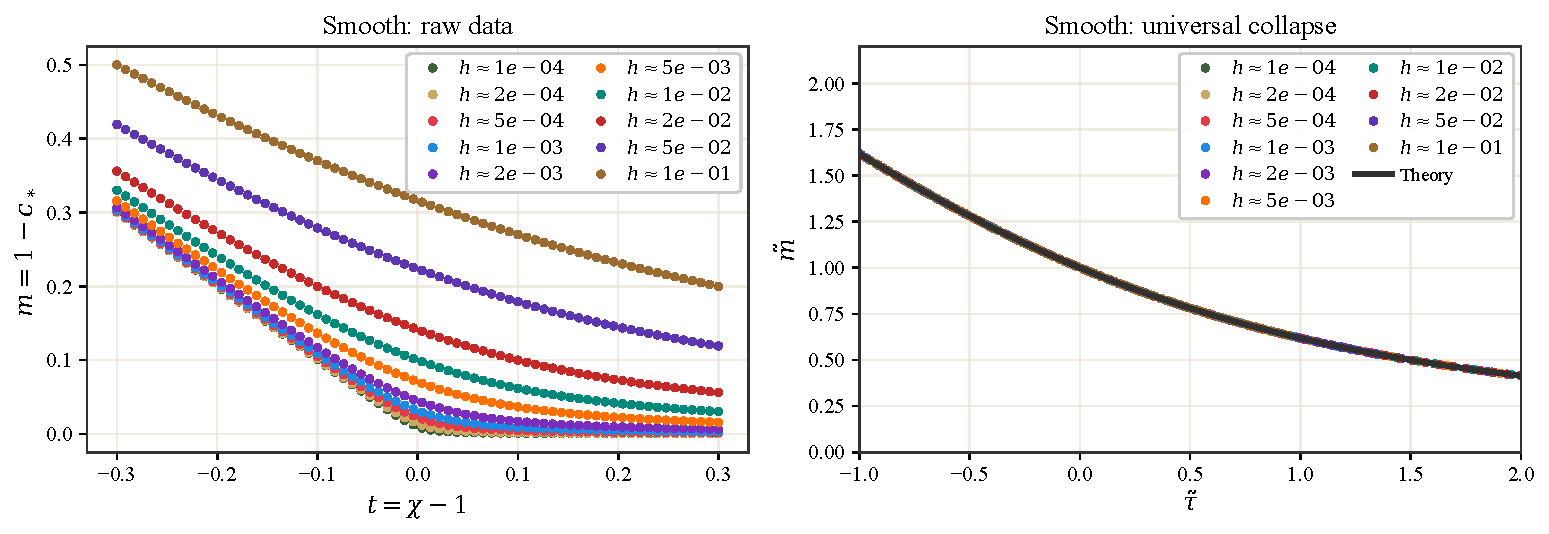
\includegraphics[width=1.0\textwidth]{figures/theory/smooth_scaling_collapse.pdf}
    \caption{
        Two-parameter crossover and scaling collapse of the dropout-deformed equation of state for the smooth universality class (tanh). Plots obtained using MFT recursion relations. The curves collapse onto a universal function after rescaling by \(\tilde t\) and \(\tilde m\). The kinked counterpart is shown in Fig.~\ref{fig:kinked_collapse}.}
    \label{fig:uni_scaling}
\end{figure*}


Figure~\ref{fig:uni_scaling} shows this collapse for smooth activations. This also clarifies the tanh/\relu{} dichotomy observed in ResNet mean-field theory \cite{yang2017meanfieldresnets}: tanh belongs to the smooth class, where the analytic \(m^2\) term makes weak fields especially important and long correlation lengths are preserved when dropout is kept small; \relu{} belongs to the kinked class, where the \(m^{3/2}\) branch point broadens the crossover window and makes the dynamics more forgiving to imperfect tuning. In short, smooth channels reward keeping the dropout field very weak, while kinked channels tolerate detuning over a wider range; neither class is uniformly preferable.










\subsection{Optimal dropout scheduling and rank-flow tie-breaking}
\label{subsec:optimal_dropout}

So far we have taken the keep probability to be constant with depth. Since dropout enters as a relevant field that cuts off the depth correlation length even at the correlation edge, it is natural to ask how to allocate a fixed dropout budget across layers so as to preserve near-critical propagation as much as possible. Let us introduce a depth-dependent keep probability $\rho_\ell$ and define the associated dropout field
%
\begin{equation}
h_\ell \;\equiv\; \Delta(\rho_\ell),
\end{equation}
%
i.e. the shift of the correlation map at perfect alignment induced by keep probability $\rho_\ell$. In the smooth universality class, linearizing the correlation map about the dropout-shifted fixed point gives (see \eqref{eq:lambda_smooth_correct})
%
\begin{equation}
\lambda(t,h_\ell)\;\simeq\; 1-\sqrt{t^2+2g_\rho h_\ell}.
\end{equation}
%
For $0<\lambda_\ell\lesssim 1$, perturbations propagate multiplicatively,
%
\begin{equation}
\delta c_L \;\sim\; \prod_{\ell=1}^L \lambda_\ell \,\delta c_0, \qquad \lambda_\ell \;\equiv\; \lambda(t,h_\ell),
\label{delta_c_dropout_perturb}
\end{equation}
%
which motivates defining an effective inverse correlation length as the mean decay rate per layer,
%
\begin{equation}
\xi_{\rm eff}^{-1} \;\equiv\; -\frac{1}{L}\sum_{\ell=1}^L \log\lambda_\ell \;\simeq\; \frac{1}{L}\sum_{\ell=1}^L \sqrt{t^2+2g_\rho h_\ell}.
\end{equation}
%
At the correlation edge $t=0$, this reduces to
%
\begin{equation}
\xi_{\rm eff}^{-1}(t=0) \;\simeq\; \sqrt{2g_\rho}\,\frac{1}{L}\sum_{\ell=1}^L h_\ell^{1/2} \;\propto\; \frac{1}{L}\sum_{\ell=1}^L h_\ell^{1/2}.
\label{eff_corr}
\end{equation}
%
We now fix a total dropout budget and local bounds,
%
\begin{equation}
\bar h \;\equiv\; \frac{1}{L}\sum_{\ell=1}^L h_\ell, \qquad 0 \le h_\ell \le h_{\max}.
\end{equation}
%
The budget above is a budget in the dropout field \(h_\ell\), not directly in the raw dropout probability \(p_{\mathrm{drop},\ell}=1-\rho_\ell\). For weak dropout,
%
\begin{equation}
\begin{aligned}
h_\ell &= a\,p_{\mathrm{drop},\ell} + \mathcal O(p_{\mathrm{drop},\ell}^2),\\
a&=\frac{\sigma_w^2}{q^\ast}\int Dz\,\phi^2(\sqrt{q^\ast}z),
\end{aligned}
\end{equation}
%
so a fixed \(h\)-budget and a fixed dropout-probability budget agree to leading order. For larger dropout, the nonlinear map \(h_\ell=\Delta(\rho_\ell)\) should be used explicitly.
Maximizing $\xi_{\rm eff}$ is equivalent to minimizing $\xi_{\rm eff}^{-1}$, so in the continuum limit ($x=\ell/L$) we obtain the constrained variational problem
%
\begin{equation}
\min_{h}\int_0^1 h(x)^{1/2}\,dx \qquad {\rm s.t.}\qquad \int_0^1 h(x)\,dx=\bar h.
\end{equation}
%
Since $h^{1/2}$ is concave, Jensen's inequality implies that any constant schedule maximizes $\int h^{1/2}$ at fixed mean; hence any minimizer must saturate the box constraint and is step-like. Equivalently, any schedule that takes values in \(\{0,h_{\max}\}\) with active fraction \(f=\bar h/h_{\max}\) is optimal for the mean-field functional. A front-loaded representative, selected below by the rank-flow tie-breaker, is
%
\begin{equation}
h(x)= \begin{cases} h_{\max}, & 0\le x\le f,\\
0, & f<x\le 1, \end{cases} \qquad f=\frac{\bar h}{h_{\max}},
\end{equation}
%
where \(x=0\) denotes the input side. All permutations of this saturated set give the same \(\xi_{\rm eff}\) in the mean-field objective; the ordering is fixed only after the beyond-mean-field tie-breaker is introduced. For this representative, uniform dropout yields $\xi_{\rm eff}\sim \bar h^{-1/2}$ while the step schedule gives
%
\begin{equation}
\frac{\xi_{\rm eff,step}}{\xi_{\rm eff,uniform}} = \sqrt{\frac{h_{\max}}{\bar h}} \;\ge\; 1.
\end{equation}
%
For kinked activations at $t=0$, one has $\xi^{-1}\propto h^{1/3}$, so the objective becomes $\int_0^1 h(x)^{1/3}dx$, which is also concave and therefore the same conclusion immediately follows. 

At the level of mean-field correlation dynamics, $\xi_{\rm eff}$ depends on $\{h_\ell\}$ only through symmetric sums (e.g. \eqref{eff_corr}), and is therefore invariant under permutations of the depth profile. Mean field fixes the optimal allocation in magnitude (step-like), but cannot by itself select which layers should receive the concentrated dropout.

In practice, this suggests a simple construction. Choose a mean-field budget $\bar h$ and a local cap $h_{\max}$, set the active fraction \(f=\bar h/h_{\max}\), and put dropout at the cap on roughly an \(f\) fraction of the layers. The correlation calculation fixes the amount of dropout but not the ordering in depth. When early coadaptation or rank collapse is the main concern, the natural tie-break is to put more of the budget near the input. In residual or transformer-like models, a linearly decreasing schedule is a smoother version of the same idea and can be preferable empirically.

The remaining tie-breaker comes from representation dynamics beyond the mean-field closure. Rank collapse gives one concrete mechanism \cite{dong2021attention,noci2022signalpropagation,daneshmand2020batch}: token diversity in pure attention decays with depth, and unnormalized MLPs can suffer analogous rank loss. By analogy with these rank-collapse mechanisms, dropout pushes in the opposite direction at the level of second moments by inflating diagonal variance and shrinking normalized correlations, thereby increasing a participation-ratio effective rank (App.~\ref{app:rank_flow}). This mechanism is preventative rather than reparative: once the representation has collapsed to an essentially one-dimensional signal subspace, inverted dropout mostly adds training-time diagonal noise rather than constructing new task-relevant modes. Thus rank flow breaks the permutation symmetry of \(\xi_{\rm eff}\) by favoring concentrated dropout where collapse is fastest; in regularization and rank-collapse-limited regimes, this means front-loading the dropout budget.

To test these predictions, we deliberately work in controlled regimes where mean-field assumptions remain valid (width $\gg$ depth, moderate dropout) rather than pursuing benchmark performance. We evaluate MLPs and Vision Transformers \cite{dosovitskiy2021vit} using CIFAR-10/100 \cite{krizhevsky2009cifar} (full details in App.~\ref{app:experimental_info}), where finite-width corrections and extensive data augmentation do not obscure the signal-propagation effects central to our analysis. Across architectures, early step-like schedules consistently outperform constant dropout (e.g., ViT on CIFAR-100: linearly decreasing achieves $49.38\%$ vs $48.69\%$ constant, $p < 0.05$), confirming that the scheduling principle transfers beyond the MLP setting in which it was derived. The appendices check that this is not a single-run effect: the gains persist across \(\bar h\)-sweeps and large-width sweeps for kinked \relu{} MLPs (App.~\ref{app:sweeps}, Fig.~\ref{fig:mlp_sweeps}), across the smooth GELU activation class (App.~\ref{app:sweeps}, Fig.~\ref{fig:gelu_h_sweep}), and across transformer schedules and component ablations (Figs.~\ref{fig:dropout_regimes_transformer} and~\ref{fig:ablations}). Table~\ref{tab:loss_improvements} summarizes the final-epoch gains. The advantage weakens only at high dropout or in overly narrow networks, precisely where the theory exits its regime of validity.

\begin{table*}[t]
\caption{Final-epoch improvements over the corresponding constant-dropout baseline. Accuracy gains are shown both as percentage-point differences and as relative percent improvements over the baseline final accuracy. Loss reductions are relative reductions in cross-entropy. Detailed appendix tables list best and final test accuracy where applicable.}
\label{tab:loss_improvements}
\centering
\scriptsize
\setlength{\tabcolsep}{4pt}
\begin{tabular}{@{}L{0.27\textwidth}L{0.23\textwidth}rrr@{}}
\toprule
\textbf{Experiment} & \textbf{Schedule} & \(\Delta\) acc. (pp) & Acc. gain & Loss reduction \\
\midrule
MLP overfitting, Fig.~\ref{fig:dropout_regimes_overfit}
& Step (early)
& \(+0.83\) & \(+2.0\%\) & \(+17.9\%\) \\
\addlinespace[1pt]
MLP budget controls, Fig.~\ref{fig:triple_dropout}
& Big step (1/3)
& \(+1.08\) & \(+2.6\%\) & \(+22.6\%\) \\
\addlinespace[1pt]
\relu{} \(h\)-sweep at \(\bar h=0.1\), Fig.~\ref{fig:mlp_sweeps}
& Big step (1/3)
& \(+2.04\) & \(+5.0\%\) & \(+35.4\%\) \\
\addlinespace[1pt]
GELU \(h\)-sweep at \(\bar h=0.1\), Fig.~\ref{fig:gelu_h_sweep}
& Big step (1/3)
& \(+0.62\) & \(+1.5\%\) & \(+29.8\%\) \\
\addlinespace[1pt]
ViT CIFAR-100, Fig.~\ref{fig:dropout_regimes_transformer}
& Linear (decreasing)
& \(+0.66\) & \(+1.4\%\) & \(+4.2\%\) \\
\addlinespace[1pt]
ViT CIFAR-10 ablations, Fig.~\ref{fig:ablations}
& Both blocks, step (early)
& \(+0.52\) & \(+0.7\%\) & \(+6.3\%\) \\
\bottomrule
\end{tabular}
\end{table*}










\section{Conclusions and further scope for research}
By extending mean-field signal propagation to include multiplicative dropout, we established that activation non-analyticity fundamentally dictates universality. This formalism yields a Landau equation of state for the decorrelation order parameter, a universal two-parameter scaling collapse, and distinct critical exponents for smooth versus kinked channels. Mean-field theory is often best at clarifying the mechanisms inside wide networks, and less often at producing directly testable design rules; here it gives one such rule. Treating dropout as a depth-dependent field leads to front-loaded schedules, which outperform constant dropout in the controlled regimes we test. Extending this mean-field analysis to attention mechanisms and incorporating finite-width corrections are natural directions for future work.










\section{Limitations}
Mean-field theory gives the leading description of MLPs at large width, with finite-width corrections controlled perturbatively by the depth-to-width ratio \(L/N\). Our experiments are deliberately carried out in this regime, but the present analysis does not compute these corrections explicitly. Although such corrections are not expected to change the smooth/kinked universality classification, they can accumulate with depth and may induce subleading changes to the optimal dropout profile.

A second limitation is architectural scope. We analyze dropout most explicitly in MLP mean-field theory, leaving full treatments of CNNs, RNNs, ResNets, Transformers, and normalization layers to future work. Still, the recursion relation is the qualitative engine behind the universality result, and analogous local Gaussian kernels appear in several wider architectures. App.~\ref{app:cnn_extension} explains why infinite-channel CNNs and residual branches should inherit much of the same smooth/kinked split, although we do not derive the full spatial-mode CNN Landau theory, run CNN experiments, or give a dropout-deformed ResNet treatment. Residual architectures are subtler because skip connections modify large-depth propagation while preserving the local activation channel. Extending the analysis to include residual-branch strength as an additional control parameter would put the Transformer experiments on firmer theoretical footing.

Third, the theory still focuses primarily on forward correlation dynamics. The main text gives the leading wide-limit backward covariance recursion and shows that dropout creates the same diagonal/off-diagonal asymmetry for gradients, but we do not develop the full dropout-deformed backward theory, including finite-width gradient susceptibilities, training-time mask correlations, or feature-learning effects. Finally, the framework is an initialization theory rather than a full theory of training dynamics: it does not model how the relevant observables evolve after feature learning substantially reshapes the representation, for instance in large-learning-rate regimes where catapult dynamics can appear \cite{zhu2024quadraticcatapult}. Extending the same approach to training-time regularizers, dropout warm-up, adaptive schedules, other regularization fields such as \(L^2\) penalties, or broader scaling-law questions \cite{Bahri2024ExplainingScalingLaws} is a natural direction for future work.










\section*{Impact statement}
The main practical benefit is improved performance at fixed training cost, or potentially reduced training cost when targeting a fixed performance level. We do not anticipate additional ethical risks.

\bibliography{bibliography}
\bibliographystyle{icml2026}



\newpage
\onecolumn


\appendix










\section{Mean-Field Background and Dropout Recursions}










\subsection{Notation guide}
\label{app:notation}

The same few letters carry several nearby meanings, so we collect the main conventions here.
\begin{table}[h]
\caption{Notation used across the main text and appendices.}
\label{tab:notation_guide}
\centering
\small
\begin{tabular}{@{}ll@{}}
\toprule
Symbol & Meaning \\
\midrule
\(\rho_\ell\) & keep probability in layer \(\ell\) \\
\(p_{\mathrm{drop},\ell}=1-\rho_\ell\) & raw dropout probability \\
\(p_j^{(\ell)}\) & Bernoulli dropout mask variable \\
\(m=1-c^\ast\) & decorrelation order parameter at the fixed point \\
\(m_\ell=1-c_\ell\) & depth-dependent decorrelation used in relaxation laws \\
\(\chi_\perp\), \(\chi_1\) & no-dropout angular susceptibility at \(c=1\) \\
\(\chi_\rho\) & dropout-deformed angular susceptibility \(\bar F_\rho'(1)\) \\
\(\chi_M\) & response susceptibility \(\partial m/\partial h\) \\
\(\chi\), \(\chi_q\) & generic Hermite/angle susceptibility and variance-channel susceptibility \\
\(\theta_{\rm rel}\) & relaxation exponent, \(m_\ell\sim \ell^{-\theta_{\rm rel}}\) \\
\bottomrule
\end{tabular}
\end{table}
\FloatBarrier










\subsection{Mean-Field Theory Primer}
\label{app:mft_primer}

Even the Standard Model of physics, with only on the order of a few dozen empirical parameters, invites the feeling that some deeper organizing principle is yet to be found. Fermi made the same point more sharply to Dyson by quoting von Neumann: ``With four parameters I can fit an elephant, and with five I can make him wiggle his trunk'' \cite{Dyson2004Fermi}. Modern machine learning pushes this worry to an extreme: parameters are abundant, so understanding cannot mean tracking each weight individually. A pressing question in modern ML literature is what set of parameters or effective fields can give a useful description of the network's behavior, and how to derive such a description from the microscopic model.

Mean-field theory gives one such effective description: instead of tracking every neuron and every random weight, one tracks a small number of self-consistent fields. In the signal-propagation version used here, those fields are variances, covariances, and correlations. This is the deep information propagation line of mean-field theory \cite{poole2016exponentialexpressivitydeepneural,schoenholz2017deepinformationpropagation}, with broader background in statistical-mechanics treatments of deep learning \cite{Bahri2020StatMechDeepLearning,bahri2024leshoucheslecturesdeep}. The same infinite-width covariance recursion can also be read as the NNGP kernel recursion \cite{Lee2018DNNasGP}; we use the MFT language because our questions concern fixed points, susceptibilities, correlation lengths, and critical exponents rather than the induced function-space prior or training dynamics.

Section~\ref{sec:mft_background} gives the main-body version of the signal-propagation story. Here we only fix notation and record the elementary steps used later in the appendices. For a depth-$L$ MLP with activation $\phi:\mathbb R\to\mathbb R$, weights and biases are initialized as
%
\begin{equation}
W^{l}_{ij}\sim \mathcal{N}\!\left(0,\frac{\sigma_{w}^{2}}{N_{l}}\right), \qquad b^{l}_{i}\sim \mathcal{N}\!\left(0,\sigma_{b}^{2}\right),
\end{equation}
%
and propagated by
%
\begin{equation}
z^{\,l}_{i;a}= W^{l}_{ij}\,y^{\,l}_{j;a}+b^{l}_{i}, \qquad y^{\,l+1}_{i;a}=\phi\!\left(z^{\,l}_{i;a}\right),
\end{equation}
%
where $a$ labels the input. We write
%
\begin{equation}
\int Dz\,(\cdots)=\frac{1}{\sqrt{2\pi}}\int_{-\infty}^{\infty}dz\,e^{-z^{2}/2}(\cdots),
\end{equation}
%
and use the same convention for multiple Gaussian variables.

The Gaussian closure comes from the fact that each preactivation is a sum of many independently initialized weighted inputs. In the infinite-width limit this central-limit effect becomes exact layer-by-layer, while finite-width corrections are organized perturbatively in the depth-to-width aspect ratio, schematically $L/N$ \cite{roberts2022principlesdeeplearningtheory}. The single-input variance and two-input covariance recursions are therefore the closed equations already quoted in Sec.~\ref{sec:mft_background}:
%
\begin{align}
q^{\,l}_{aa}&=\sigma_{w}^{2}\int Dz\,\phi^{2}\!\left(\sqrt{q^{\,l-1}_{aa}}\,z\right)+\sigma_{b}^{2},\nonumber\\
q^{\,l}_{ab}&=\sigma_{w}^{2}\int Dz_{1}\,Dz_{2}\,\phi(u_{1})\,\phi(u_{2})+\sigma_{b}^{2},\nonumber\\
u_{1}&=\sqrt{q^{\,l-1}_{aa}}\,z_{1},\qquad c^{\,l-1}_{ab}=\frac{q^{\,l-1}_{ab}}{\sqrt{q^{\,l-1}_{aa}\,q^{\,l-1}_{bb}}},\nonumber\\
u_{2}&=\sqrt{q^{\,l-1}_{bb}}\left(c^{\,l-1}_{ab}z_{1}+\sqrt{1-\left(c^{\,l-1}_{ab}\right)^{2}}\,z_{2}\right).
\end{align}
%
Once the variance relaxes to $q^*$, these equations induce a one-dimensional correlation map $c^l_{ab}=F(c^{l-1}_{ab})$. Without dropout, perfect alignment is a fixed point, $F(1)=1$. Its linear stability is controlled by the angular susceptibility
%
\begin{equation}
\chi_{1}=\left.\frac{\partial c^{\,l}_{ab}}{\partial c^{\,l-1}_{ab}}\right|_{c_{ab}=1}=\sigma_{w}^{2}\int Dz\,\big[\phi'(\sqrt{q^{*}}\,z)\big]^{2},
\end{equation}
%
called $\chi_\perp$ in the main text and in \cite{roberts2022principlesdeeplearningtheory}. The ordered, chaotic, and critical regimes correspond to $\chi_1<1$, $\chi_1>1$, and $\chi_1=1$ respectively; the last case is the edge-of-chaos, where the cross-input correlation length can diverge.

The usual He initialization follows from this criterion in the special case of \relu{}. Since $\phi'(z)=\theta(z)$ almost everywhere,
%
\begin{equation}
\int Dz\,\big(\phi'(\sqrt{q^{*}}z)\big)^2=\frac12,
\qquad \chi_1=1 \Longrightarrow \sigma_w^2=2,
\end{equation}
%
which is the variance-$2/N$ initialization. The same example also shows why variance preservation and correlation criticality are not identical: for \relu{},
%
\begin{equation}
q^{\,l}_{aa}=\frac{\sigma_w^2}{2}\,q^{\,l-1}_{aa}+\sigma_b^2,
\end{equation}
%
so with nonzero bias the finite-$q^*$ condition requires $\sigma_w^2<2$, while exact angular criticality sets $\sigma_w^2=2$. In practice one either sets biases to zero or works slightly subcritical to keep the variance scale finite.

Finally, the correlation length used throughout the paper is obtained by linearizing the correlation map around its fixed point. If $r_c=F'(c^*)$, then
%
\begin{equation}
|c^*-c^l_{ab}|\propto e^{-l/\xi_c},\qquad \xi_c^{-1}=-\log|r_c|.
\end{equation}
%
The analogous variance length $\xi_q$ tracks relaxation of $q^l_{aa}$ to $q^*$, but the edge-of-chaos phenomenon is primarily controlled by $\xi_c$: it measures how many layers preserve distinctions between different inputs. This is the scale deformed by dropout in the main analysis.
\FloatBarrier










\subsection{Derivation of Correlation Map and Derivatives with Dropout}\label{app:price_dropout}

This subsection supplies the steps leading to Eqs.~\eqref{eq:chi_dropout} and \eqref{eq:g_dropout}, starting from the two-input correlation recursion that underlies the perfect-alignment shift \(\bar F_\rho(1)=1-\Delta\) in \eqref{eq:Delta_exact}.


Fix a layer where the single-input variance has converged to the dropout-shifted fixed point \(\bar q^*\) defined by \eqref{eq:qstar-dropout}. For two inputs, let \((u_1,u_2)\) be jointly Gaussian with
%
\begin{equation}
\mathbb E[u_1^2]=\mathbb E[u_2^2]=\bar q^*, \qquad \mathbb E[u_1u_2]=c\,\bar q^*, \qquad c\in[-1,1].
\end{equation}
%
The normalized correlation map is
%
\begin{equation}
\bar F_\rho(c) \;\equiv\; \frac{\bar q^{l+1}_{ab}}{\bar q^*} \;=\; \frac{\sigma_w^2\,\mathbb E\!\big[\phi(u_1)\phi(u_2)\big]+\sigma_b^2}{\bar q^*}.
\label{eq:Frho_def_app}
\end{equation}
%
At \(c=1\), \(u_1=u_2\) and \(\bar F_\rho(1)=1-\Delta\) by definition, giving \eqref{eq:Delta_exact}.


Since \(\bar q^*\) is independent of \(c\), differentiating \eqref{eq:Frho_def_app} yields
%
\begin{equation}
\bar F_\rho'(c) \;=\; \frac{\sigma_w^2}{\bar q^*}\, \frac{\partial}{\partial c}\, \mathbb E\!\big[\phi(u_1)\phi(u_2)\big].
\label{eq:Frho_prime_step1}
\end{equation}
%
Write \(u_i=\sqrt{\bar q^*}\,v_i\), where \((v_1,v_2)\) are standard Gaussians with \(\mathbb E[v_1v_2]=c\), and define
%
\begin{equation}
G(c)\;\equiv\;\mathbb E\!\Big[\phi\!\big(\sqrt{\bar q^*}\,v_1\big)\,\phi\!\big(\sqrt{\bar q^*}\,v_2\big)\Big].
\end{equation}
%
Price's theorem \cite{Price1958GaussianInputs} gives
%
\begin{equation}
\frac{\mathrm d}{\mathrm dc}G(c) \;=\; \mathbb E\!\left[ \frac{\partial^2}{\partial v_1\,\partial v_2} \Big( \phi\!\big(\sqrt{\bar q^*}\,v_1\big)\, \phi\!\big(\sqrt{\bar q^*}\,v_2\big) \Big) \right].
\label{eq:price_step}
\end{equation}
%
A direct differentiation yields
%
\begin{equation}
\frac{\partial^2}{\partial v_1\,\partial v_2} \Big( \phi\!\big(\sqrt{\bar q^*}\,v_1\big)\, \phi\!\big(\sqrt{\bar q^*}\,v_2\big) \Big) = \bar q^*\, \phi'\!\big(\sqrt{\bar q^*}\,v_1\big)\, \phi'\!\big(\sqrt{\bar q^*}\,v_2\big).
\end{equation}
%
Therefore,
%
\begin{equation}
G'(c) = \bar q^*\, \mathbb E\!\Big[ \phi'\!\big(\sqrt{\bar q^*}\,v_1\big)\, \phi'\!\big(\sqrt{\bar q^*}\,v_2\big) \Big].
\end{equation}
%
Taking \(c\to 1\) collapses \(v_1=v_2=z\) with \(z\sim\mathcal N(0,1)\), hence
%
\begin{equation}
G'(1) = \bar q^*\int Dz\,\big[\phi'(\sqrt{\bar q^*}\,z)\big]^2.
\end{equation}
%
Substituting into \eqref{eq:Frho_prime_step1} gives
%
\begin{equation}
\bar F_\rho'(1) = \sigma_w^2\int Dz\,\big[\phi'(\sqrt{\bar q^*}\,z)\big]^2,
\end{equation}
%
which is Eq.~\eqref{eq:chi_dropout}. Differentiating \eqref{eq:Frho_prime_step1} once more:
%
\begin{equation}
\bar F_\rho''(c) \;=\; \frac{\sigma_w^2}{\bar q^*}\, \frac{\partial^2}{\partial c^2}\, \mathbb E\!\big[\phi(u_1)\phi(u_2)\big].
\label{eq:Frho_second_step1}
\end{equation}
%
Applying Price's theorem again to
\(
f(v_1,v_2)=\phi'(\sqrt{\bar q^*}\,v_1)\phi'(\sqrt{\bar q^*}\,v_2)
\)
yields
%
\begin{equation}
\frac{\mathrm d}{\mathrm dc} \mathbb E\!\Big[ \phi'(\sqrt{\bar q^*}\,v_1)\phi'(\sqrt{\bar q^*}\,v_2) \Big] = \bar q^*\, \mathbb E\!\Big[ \phi''(\sqrt{\bar q^*}\,v_1)\phi''(\sqrt{\bar q^*}\,v_2) \Big].
\end{equation}
%
Combining with the previous step gives
%
\begin{equation}
\frac{\partial^2}{\partial c^2}\, \mathbb E\!\big[\phi(u_1)\phi(u_2)\big] = (\bar q^*)^2\, \mathbb E\!\Big[ \phi''(\sqrt{\bar q^*}\,v_1)\phi''(\sqrt{\bar q^*}\,v_2) \Big].
\end{equation}
%
Evaluating at \(c=1\) again collapses \(v_1=v_2=z\), so
%
\begin{equation}
\left.\frac{\partial^2}{\partial c^2}\, \mathbb E\!\big[\phi(u_1)\phi(u_2)\big]\right|_{c=1} = (\bar q^*)^2\int Dz\,\big[\phi''(\sqrt{\bar q^*}\,z)\big]^2.
\end{equation}
%
Substituting into \eqref{eq:Frho_second_step1} yields
%
\begin{equation}
\bar F_\rho''(1) = \sigma_w^2\,\bar q^*\int Dz\,\big[\phi''(\sqrt{\bar q^*}\,z)\big]^2,
\end{equation}
%
which is Eq.~\eqref{eq:g_dropout}.

\FloatBarrier










\subsection{Extensions to Infinite-Channel CNNs and ResNets}
\label{app:cnn_extension}

We briefly discuss extensions to architectures not treated in the main analysis. Although our derivation is for MLPs, the universality-class mechanism is tied to the local Gaussian kernel rather than to the MLP architecture itself. Other architectures introduce additional structure that can change the exact exponents, but the qualitative smooth-versus-kinked distinction should remain when the same local channel controls the wide-limit recursion. 

For example, the same local channel which appears in MLPs re-emerges in infinite-width CNNs when the number of channels is taken to infinity: preactivations at different spatial positions become jointly Gaussian across channels, and the covariance recursion composes the same bivariate Gaussian activation expectation with a linear operator that averages over convolutional filter offsets \cite{cnnslecun,xiao2018dynamicalisometrymeanfield}. In schematic form, a spatial covariance \(K^\ell_{\alpha\beta}(x,x')\) evolves as \(K^{\ell+1}=\sigma_b^2+\sigma_w^2\mathcal A[V_\phi(K^\ell)]\), where \(V_\phi\) is the scalar Gaussian channel analyzed above and \(\mathcal A\) is the convolutional averaging operator. Independent dropout shifts the single-input variance entering \(V_\phi\) as in the fully connected case, while the cross-input covariance is still controlled by the same bivariate expectation. Therefore, for an isolated leading spatial mode, convolution changes the relevant eigenvalue and mode shape but not the local smooth-versus-kinked non-analyticity: smooth activations retain the analytic Landau equation, while \relu{}-like kinks retain the \(m^{3/2}\) branch point. A complete CNN theory would promote \(m\) to a spatial covariance-mode amplitude and track boundary conditions, pooling, and degeneracies of \(\mathcal A\).

ResNets modify depth dynamics in a complementary way: skip connections can change exponential convergence to subexponential or polynomial behavior, and norms may drift rather than relax to a fixed point \cite{yang2017meanfieldresnets}. Still, the residual branch evaluates the same nonlinear Gaussian channel \(V_\phi\), so the local analytic distinction is unchanged. The tanh/\relu{} asymptotic split observed in \cite{yang2017meanfieldresnets} is consistent with our smooth/kinked classes; a dropout-deformed ResNet theory would additionally track residual-branch strength and norm drift.

\FloatBarrier










\subsection{Rank Collapse and Rank-Flow Tie-Breaking}
\label{app:rank_flow}

The mean-field propagation objective is invariant under permutations of the depth profile \(h_\ell\), so it fixes the amount of dropout but not its ordering. Rank collapse supplies one beyond-mean-field tie-breaker \cite{dong2021attention,noci2022signalpropagation,daneshmand2020batch}. In pure self-attention, for token representations \(X_\ell\in\mathbb R^{n\times d}\), and ignoring residual connections, \(X_{\ell+1}=A_\ell X_\ell\). Hence
%
\begin{equation}
\operatorname{rank}(X_{\ell+1}) \;\leq\; \min\{\operatorname{rank}(A_\ell),\operatorname{rank}(X_\ell)\}.
\end{equation}
%
As \(A_\ell\) contracts toward the rank-one projector \(\mathbf 1\mathbf 1^\top/n\), a rank-diversity proxy normalized so that \(R=1\) at complete token collapse obeys
%
\begin{equation}
R(\ell)-1 \;\lesssim\; \bigl(R(0)-1\bigr)\exp\!\left(-c\,2^\ell\right),
\end{equation}
%
for an architecture-dependent constant \(c>0\). Unnormalized MLPs show a related rank-collapse mechanism: products of random linear maps converge toward a rank-one direction at an exponential rate, while \relu{} MLPs exhibit fast rank loss empirically \cite{daneshmand2020batch}. A simple proxy for the linear case is
%
\begin{equation}
R(\ell)-1 \;\sim\; \bigl(R(0)-1\bigr)\exp\!\left(-2(\lambda_1-\lambda_2)\,\ell\right),
\end{equation}
%
where $\lambda_1>\lambda_2$ are the top Lyapunov exponents governing singular-value growth. In both cases, the dominant loss of diversity occurs early in depth, especially in attention-dominated models.

Dropout counteracts this collapse by shrinking within-layer normalized correlations. With keep probability $\rho_\ell\in(0,1]$, inverted dropout acts as
%
\begin{equation}
\tilde y_{\ell,i} \;=\; \frac{p_{\ell,i}}{\rho_\ell}\,y_{\ell,i}, \qquad p_{\ell,i}\sim \mathrm{Bernoulli}(\rho_\ell),
\end{equation}
%
with the $p_{\ell,i}$ independent across $i$. Let the uncentered second moment at depth $\ell$ be
%
\begin{equation}
\Sigma_\ell \;\equiv\; \mathbb{E}\!\left[y_\ell y_\ell^\top\right],
\end{equation}
%
and define $\tilde\Sigma_\ell$ analogously for $\tilde y_\ell$. Averaging over the dropout mask gives
%
\begin{equation}
\tilde\Sigma_\ell \;=\; \Sigma_\ell + \left(\frac{1}{\rho_\ell}-1\right)\mathrm{diag}(\Sigma_\ell),
\label{eq:dropout_second_moment}
\end{equation}
%
so off-diagonal second moments are unchanged while the diagonal is inflated. Writing
%
\begin{equation}
D_\ell \;\equiv\; \mathrm{diag}(\Sigma_\ell), \qquad C_\ell \;\equiv\; D_\ell^{-1/2}\Sigma_\ell D_\ell^{-1/2},
\end{equation}
%
one obtains
%
\begin{equation}
\tilde C_\ell \;=\; \rho_\ell\,C_\ell + (1-\rho_\ell)\,I.
\label{eq:dropout_corr_shrinkage}
\end{equation}
%
This identity suppresses off-diagonal correlations and moves the eigenvalues of the normalized correlation matrix \(C_\ell\) toward one. The statement is about the normalized correlation matrix; the raw covariance \(\tilde\Sigma_\ell\) can still have heterogeneous diagonal variances.

A convenient quantitative proxy is the participation-ratio effective rank
%
\begin{equation}
R_{\mathrm{eff}}(\Sigma) \;\equiv\; \frac{\bigl(\mathrm{tr}\,\Sigma\bigr)^2}{\mathrm{tr}\!\left(\Sigma^2\right)}.
\end{equation}
%
Combining \eqref{eq:dropout_second_moment} with trace identities yields
%
\begin{equation}
R_{\mathrm{eff}}\!\left(\tilde\Sigma_\ell\right) \;=\; \frac{\bigl(\mathrm{tr}\,\Sigma_\ell\bigr)^2}{ \rho_\ell^2\,\mathrm{tr}\!\left(\Sigma_\ell^2\right) + \left(1-\rho_\ell^2\right)\mathrm{tr}\!\left(\mathrm{diag}(\Sigma_\ell)^2\right)}.
\end{equation}
%
Since $\mathrm{tr}(\Sigma_\ell^2)\ge \mathrm{tr}(\mathrm{diag}(\Sigma_\ell)^2)$ for any PSD $\Sigma_\ell$,
%
\begin{equation}
R_{\mathrm{eff}}\!\left(\tilde\Sigma_\ell\right)\;\ge\;R_{\mathrm{eff}}(\Sigma_\ell),
\end{equation}
%
with equality iff \(\rho_\ell=1\) or \(\Sigma_\ell\) is diagonal (equivalently, for any nontrivial dropout \(0<\rho_\ell<1\), iff all off-diagonal entries vanish). Independent additive noise would also inflate the diagonal and break perfect alignment; dropout is the multiplicative Bernoulli realization for which the effective field is directly controlled by $\rho_\ell$.

\FloatBarrier










\section{Critical Exponents and Non-Analyticity}
\label{ap:exponent_derivations}

The Hermite decomposition in App.~\ref{sec:hermite} diagnoses which expansion is valid here. In the Gaussian channel,
%
\begin{equation}
F(c)=\frac{\sigma_w^2\sum_{n\ge0}a_n^2 c^n+\sigma_b^2}{q^*}.
\end{equation}
%
Rapid Hermite decay makes this series analytic at \(c=1\), giving the ordinary Taylor/Landau equation below. A kink produces a power-law Hermite tail, so high-degree modes contribute collectively as \(c\to1\); the Taylor expansion is replaced by the branch-point term \(m^{3/2}\), which is the source of the kinked exponents.










\subsection{Smooth Networks}

The standard static exponents follow directly from \eqref{eq:EoS_correct}. Along the critical isotherm \(t=0\),
%
\begin{equation}
h=\frac{g_\rho}{2}m^2 \qquad\Rightarrow\qquad m\sim h^{1/2},
\end{equation}
%
so \(\delta=2\). The analogue of the magnetic susceptibility is \(\chi_M(t)\equiv \left.\partial m/\partial h\right|_{h\to 0}\).
On the subcritical side \(t<0\), the analytic branch satisfies \(m\simeq -h/t\), hence \(\chi_M(t)\sim |t|^{-1}\) and \(\gamma=1\).
Along \(h=0\), the physical branch is \(m=0\) for \(t\le 0\) and \(m=2t/g_\rho\) for \(t\ge 0\), so \(m\sim t\) as \(t\to 0^+\) and \(\beta=1\).

\vspace{0.25em}
\noindent
The depth correlation length follows from linearizing the correlation dynamics about the displaced fixed point.
To leading order,
%
\begin{equation}
\lambda \equiv \bar F_\rho'(c^*) = \bar F_\rho'(1-m)\simeq \chi_\rho-g_\rho m = 1+t-g_\rho m,
\end{equation}
%
and substituting \eqref{eq:m_smooth_solution} gives
%
\begin{equation}
\lambda(t,h)=1-\sqrt{t^2+2g_\rho h}.
\label{eq:lambda_smooth_correct}
\end{equation}
%
For \(\lambda\simeq 1\) with \(\lambda>0\), the depth correlation length satisfies
%
\begin{equation}
\xi_{c,\rho}^{-1}\equiv -\log\lambda \simeq 1-\lambda = \sqrt{t^2+2g_\rho h}.
\end{equation}
%
Thus \(\xi_{c,\rho}(t,0)\sim |t|^{-1}\) and \(\nu_t=1\), while \(\xi_{c,\rho}(0,h)\sim h^{-1/2}\) and \(\nu_\rho=1/2\).
Equivalently, \(y_t=1/\nu_t=1\) and \(y_\rho=1/\nu_\rho=2\), so dropout is the more relevant perturbation of the correlation edge.

At the marginal point \(t=h=0\), the same smooth normal form gives the depth relaxation law:
%
\begin{equation}
m_{\ell+1}-m_\ell\simeq-\frac{g_\rho}{2}m_\ell^2.
\end{equation}
%
In a continuum-depth approximation this gives \(m(\ell)\sim \ell^{-1}\), hence \(\theta_{\rm rel}=1\) for the smooth class.

\vspace{0.25em}
\noindent
A pseudo-free-energy functional consistent with \eqref{eq:EoS_correct} is
%
\begin{equation}
f(t,m;h) = -\frac{t}{2}\,m^2 + \frac{g_\rho}{6}\,m^3 - h\,m,
\label{eq:free_energy_correct}
\end{equation}
%
since \(\partial f/\partial m=0\) is equivalent to \eqref{eq:EoS_correct}. This object should be read in the same spirit as a low-order one-particle-irreducible (1PI) effective action: it is not a literal training loss or microscopic energy, but an effective potential for the slow variable \(m\). Its stationarity condition gives the equation of state, while its on-shell singular part organizes the thermodynamic-style exponents; analytic \(m\)-independent backgrounds can be added without changing the physics of the recursion.

At \(h=0\), substituting the physical branch
\(m=0\) for \(t\le 0\) and \(m=2t/g_\rho\) for \(t\ge 0\) yields
%
\begin{equation}
f_{\rm on}(t,0)=0 \quad (t\le 0), \qquad f_{\rm on}(t,0)=-\frac{2}{3g_\rho^{2}}\,t^{3}\quad (t\ge 0).
\end{equation}
%
Therefore the analogue of the specific heat, \(C\equiv -\partial_t^{2} f_{\rm on}\), stays finite and vanishes linearly:
%
\begin{equation}
C(t)=\frac{4}{g_\rho^{2}}\,t\,\Theta(t)\sim |t|,
\end{equation}
%
where $\Theta(t)$ is the Heaviside step function.  In standard exponent language \(C_{\rm sing}(t)\sim |t|^{-\alpha}\), this corresponds to
%
\begin{equation}
\alpha=-1,
\end{equation}
%
up to an additive analytic background \(f_0(t,h)\) that does not affect the equation of state.

Collecting exponents for the smooth universality class:
%
\begin{equation}
\beta=1, \qquad \gamma=1, \qquad \delta=2, \qquad \nu_t=1, \qquad \nu_\rho=\frac{1}{2}, \qquad \theta_{\rm rel}=1, \qquad \alpha=-1.
\end{equation}
%
For comparison, standard Ising-like Landau mean-field theory (with \(m\to -m\) symmetry and a quartic interaction) has
%
\begin{equation}
\beta=\frac{1}{2}, \qquad \gamma=1, \qquad \delta=3, \qquad \nu=\frac{1}{2}, \qquad \alpha=0.
\end{equation}
%
Our dropout-deformed correlation-edge theory shares \(\gamma=1\), but the lack of a \(\mathbb Z_2\) symmetry (and the resulting cubic interaction)
shifts \(\beta\) and \(\delta\), produces \(\nu_t=1\) rather than \(\nu=1/2\), and yields a specific-heat analogue that vanishes at the transition (\(\alpha=-1\))
rather than exhibiting the Ising mean-field behavior (\(\alpha=0\)).










\subsection{Kinked Networks}
\label{sec:kinks}

Up to now, the Landau-style expansion of \(\bar F_\rho(c)\) around \(c=1\) relied on the assumption that \(\bar F_\rho(c)\) is analytic in
%
\begin{equation}
m \equiv 1-c.
\end{equation}
%
For smooth activations this is the natural situation, and the first nonlinear correction is of order \(m^2\), controlled by
%
\begin{equation}
g_\rho \propto \int Dz\,\bigl[\phi''(\sqrt{\bar q^{*}}\,z)\bigr]^2.
\end{equation}
%
For kinked activations, this logic fails: the map remains smooth for \(c<1\), but as it approaches \(c\to 1\), it is governed by a branch point, and the leading nonlinear correction is non-analytic in \(m\). This changes the scaling of the dropout deformation.

We illustrate this explicitly for the \relu{} activation \(\phi(x)=\max(0,x)\). To keep formulas compact we set \(\sigma_b = 0\)
throughout this subsection and use the same inverted-dropout convention as before, with masks drawn independently across inputs.

The mean-field correlation map for \relu{} admits the standard arc-cosine closed form \cite{ChoSaul2009ArcCosine}. Writing \(c\in[-1,1]\) for the preactivation correlation at some depth,
%
\begin{align}
F_{\ReLU}(c) &= \frac{1}{\pi} \Bigl[ \sqrt{1-c^{2}} + \bigl(\pi-\cos^{-1}c\bigr)c \Bigr].
\label{eq:relu_map_rho1}
\end{align}
%
Near perfect alignment, setting \(c=1-m\) with \(0<m\ll 1\), one obtains the non-analytic expansion
%
\begin{align}
F_{\ReLU}(1-m) &= 1-m+\kappa\,m^{3/2}+{\cal O}(m^{2}),
\label{eq:relu_expand}\\
\kappa &\equiv \frac{2\sqrt{2}}{3\pi}. \nonumber
\end{align}
%
Thus, the Taylor expansion valid for smooth activations would have missed the \(m^{3/2}\) contribution. 

We now turn on dropout and again view dropout as a field deformation at \(c=1\):
%
\begin{equation}
\bar F_\rho(1)=1-h, \qquad h>0.
\end{equation}
%
In the present \(\sigma_b=0\) setting, this field is exactly
%
\begin{equation}
h \;=\; 1-\bar F_\rho(1) \;=\; 1-\rho,
\label{eq:relu_h_correct}
\end{equation}
%
independent of the activation, since at \(c=1\) the only source of mismatch is the independence of the two dropout masks.
We write the fixed point as \(c^*=1-m^*\) with \(m^*>0\) and impose \(c^*=\bar F_\rho(c^*)\).
For the literal bias-free \relu{} map, \(\bar F_\rho(c)=\rho F_{\ReLU}(c)\), so \(\chi_\rho=\rho\) and \(t=\rho-1=-h\). Thus the \(t=0,h>0\) direction below is the kinked normal-form field direction, while standard \relu{} dropout follows a constrained path through the same scaling function.

Near \(m^*\ll 1\), the kinked analogue of the Landau equation of state is obtained by combining the shift \(\bar F_\rho(1)=1-h\), the linear slope \(\chi_\rho=1+t\), and the non-analytic term \eqref{eq:relu_expand}:
%
\begin{equation}
h \;=\; \kappa\,m^{3/2} - t\,m + \mathcal O(m^2), \qquad t\equiv \chi_\rho-1.
\label{eq:eos_kink_correct}
\end{equation}
%
Along the normal-form critical isotherm \(t=0\), this gives
%
\begin{equation}
m^* \;\sim\; \left(\frac{h}{\kappa}\right)^{2/3}, \qquad (t=0),
\label{eq:kink_mstar}
\end{equation}
%
so the smooth exponent \(\delta=2\) is replaced by
%
\begin{equation}
m \propto h^{1/\delta_{\mathrm{kink}}}, \qquad \delta_{\mathrm{kink}}=\frac{3}{2}.
\label{eq:kink_delta}
\end{equation}
%
And with this we immediately find the smoking gun telling us that kinked and smooth activations fall into distinct mean-field universality classes under the dropout deformation. As before, the depth scale follows from linearizing the correlation dynamics around \(c^*\). Differentiating \eqref{eq:relu_expand} gives
%
\begin{equation}
\lambda \equiv \bar F_\rho'(c^*) \simeq 1+t-\frac{3\kappa}{2}\sqrt{m^*}.
\label{eq:kink_slope}
\end{equation}
%
At \(t=0\) we therefore have
%
\begin{equation}
1-\lambda \propto \sqrt{m^*}\propto h^{1/3}.
\end{equation}
%
Using \(\xi_{c,\rho}^{-1}\simeq 1-\lambda\) for \(\lambda\simeq 1\) yields
%
\begin{equation}
\xi_{c,\rho}(0,h) \sim h^{-1/3}, \qquad \nu_{\rho,\mathrm{kink}}=\frac{1}{3},
\label{eq:kink_nu}
\end{equation}
%
to be compared with the smooth result \(\xi_{c,\rho}(0,h)\sim h^{-1/2}\).
For ordinary bias-free \relu{} dropout, substituting the constrained path \(t=-h\) into \eqref{eq:eos_kink_correct} gives
%
\begin{equation}
h=\kappa m^{3/2}+hm+\mathcal O(m^2).
\end{equation}
%
Since the leading solution has \(m\sim h^{2/3}\), the \(hm\) term is subleading. Moreover,
%
\begin{equation}
1-\lambda\simeq h+\frac{3\kappa}{2}\sqrt m\sim h^{1/3},
\end{equation}
%
so the same \(\nu_{\rho,\mathrm{kink}}=1/3\) survives as a constrained-path exponent.

The remaining kinked exponents follow from the same equation of state. At \(h=0\) and \(t>0\),
%
\begin{equation}
\kappa m^{3/2}=tm \qquad\Rightarrow\qquad m=\left(\frac{t}{\kappa}\right)^2,
\end{equation}
%
so \(\beta_{\rm kink}=2\). On the subcritical side \(t<0\), the small-field balance is \(h\simeq |t|m\), giving \(\chi_M\sim |t|^{-1}\) and therefore \(\gamma_{\rm kink}=1\). Substituting the zero-field branch into \eqref{eq:kink_slope} gives \(1-\lambda\propto t\), so \(\xi_{c,\rho}(t,0)\sim t^{-1}\) and \(\nu_{t,\rm kink}=1\).

Adding nonzero \relu{} bias variance does not restore a finite-\(q^*\) critical isotherm. With inverted dropout,
%
\begin{equation}
\bar q_{\ell+1}=\frac{\sigma_w^2}{2\rho}\bar q_\ell+\sigma_b^2,
\end{equation}
%
so finite variance requires \(a\equiv\sigma_w^2/(2\rho)<1\), while angular criticality requires \(\chi_\rho=\sigma_w^2/2=1\), incompatible with \(\rho<1\). Equivalently, \(h=a(1-\rho)\) and \(t=\rho a-1=-h-(1-a)\), so finite variance adds a subcritical detuning that cuts off the asymptotic dropout law unless one takes the singular double scaling \(1-a\ll h^{1/3}\).



It is also useful, in direct analogy with the smooth case, to package \eqref{eq:eos_kink_correct} into a pseudo-free-energy.
A functional whose stationarity condition reproduces the kinked equation of state is
%
\begin{equation}
f_{\mathrm{kink}}(t,m;h) \;=\; -\frac{t}{2}\,m^2 + \frac{2\kappa}{5}\,m^{5/2} - h\,m,
\label{eq:free_energy_kink}
\end{equation}
%
since $\partial f_{\mathrm{kink}}/\partial m=0$ gives $h=\kappa m^{3/2}-tm$ at leading order. In the effective-action language, the \(m^{5/2}\) term is the pseudo-free-energy avatar of the branch point in the \relu{} correlation map; this is precisely where the kinked universality class departs from the analytic Landau polynomial above.\footnote{
As before, $f_{\mathrm{kink}}$ is defined only up to addition of an $m$-independent analytic background $f_0(t,h)$, which does not affect the equation of state.
}
At zero field the physical branch is $m=0$ for $t\le 0$ and $m=(t/\kappa)^2$ for $t\ge 0$, so the on-shell free energy behaves as
%
\begin{equation}
f_{\mathrm{kink,on}}(t,0)=0 \quad (t\le 0), \qquad f_{\mathrm{kink,on}}(t,0)=-\frac{1}{10\kappa^{4}}\,t^{5}\quad (t\ge 0).
\end{equation}
%
Thus the analogue of the specific heat, $C\equiv-\partial_t^{2} f_{\mathrm{kink,on}}$, stays finite and in fact vanishes as
%
\begin{equation}
C(t)\;=\;\frac{2}{\kappa^{4}}\,t^{3}\,\Theta(t)\;\sim\;|t|^{3}.
\end{equation}
%
In the standard exponent convention $C_{\mathrm{sing}}(t)\sim |t|^{-\alpha}$, this corresponds to
%
\begin{equation}
\alpha_{\mathrm{kink}}=-3.
\end{equation}
%
Although we used \relu{} to compute the near-alignment expansion in closed form, the resulting fractional power is not a peculiarity of \relu{}. Rather, it is a generic feature of the mean-field Gaussian channel whenever the activation has an ordinary kink: \(\phi\) is continuous and piecewise \(C^{1}\) with a finite jump in slope at some point. In that case the correlated-Gaussian expectation defining the normalized correlation map remains smooth for \(c<1\), but its approach to \(c\to 1\) is controlled by a square-root branch associated with the thin Gaussian tube around the diagonal \(u_{1}=u_{2}\). Writing \(c=1-m\) with \(0<m\ll 1\), the transverse fluctuations scale as \(\sqrt{m}\), so the probability that two nearly aligned preactivations fall on opposite sides of the kink scales as \(\mathcal O(\sqrt{m})\); in that straddling region a finite-slope kink produces activation mismatches of size \(\mathcal O(\sqrt{m})\), so the leading non-linear correction to the kernel scales as \(\mathcal O(\sqrt{m})\times \mathcal O(m)=\mathcal O(m^{3/2})\). Thus, for any standard kinked activation one expects
%
\begin{equation}
F(1-m)=1-m+\kappa_{\phi}\,m^{3/2}+{\cal O}(m^{2}),
\end{equation}
%
with an activation-dependent coefficient \(\kappa_{\phi}\), while the exponent \(3/2\) is fixed by the tube geometry.

Finally, it is useful to recall what happens when dropout is switched off exactly at the marginal point. Setting
%
\begin{equation}
\rho=1, \qquad t=0,
\end{equation}
%
the non-analytic correction controls the approach to \(c=1\). Writing \(m_\ell\equiv 1-c_\ell\) and using \eqref{eq:relu_expand},
%
\begin{equation}
m_{\ell+1}-m_\ell \simeq -\kappa\,m_\ell^{3/2}.
\label{eq:kink_relax}
\end{equation}
%
In a continuum-depth approximation \(m_{\ell+1}-m_\ell\to \partial_\ell m\), we obtain
%
\begin{equation}
\partial_\ell m \simeq -\kappa\,m^{3/2} \qquad\Rightarrow\qquad m(\ell)\sim \ell^{-2},
\label{eq:kink_relax_sol}
\end{equation}
%
which reproduces the characteristic \(1-c_\ell\sim \ell^{-2}\) relaxation of \relu{} activations at the edge-of-chaos \cite{hayou2019impact} and gives \(\theta_{\rm rel}=2\).










\subsection{Non-Analytic Expansion of the \relu{} Correlation Map near $c=1$}
\label{app:relu_non-analytic}

Here we derive the non-analytic expansion
%
\begin{align}
F_{\ReLU}(1-m) = 1-m+\kappa\,m^{3/2}+{\cal O}(m^{2}), \qquad \kappa=\frac{2\sqrt{2}}{3\pi},
\label{eq:app_relu_expand}
\end{align}
%
starting from the closed form \relu{} correlation map \cite{ChoSaul2009ArcCosine}
%
\begin{align}
F_{\ReLU}(c) &= \frac{1}{\pi} \Bigl[ \sqrt{1-c^{2}} + \bigl(\pi-\cos^{-1}c\bigr)c \Bigr], \qquad c\in[-1,1].
\label{eq:app_relu_map}
\end{align}
%
Set $c=1-m$ with $0<m\ll 1$.

First expand the square root term,
%
\begin{align}
\sqrt{1-c^{2}}&=\sqrt{1-(1-m)^2}=\sqrt{2m-m^{2}}=\sqrt{2m}\,\sqrt{1-\frac{m}{2}}\nonumber\\
&=\sqrt{2m}\left(1-\frac{m}{4}+{\cal O}(m^{2})\right)=\sqrt{2}\,m^{1/2}-\frac{\sqrt{2}}{4}m^{3/2}+{\cal O}(m^{5/2}).
\label{eq:app_relu_sqrt}
\end{align}
%
Next expand $\cos^{-1}(1-m)$. Write $\theta=\cos^{-1}(1-m)$ and use
%
\begin{align}
\cos\theta = 1-\frac{\theta^{2}}{2}+\frac{\theta^{4}}{24}+{\cal O}(\theta^{6}),
\label{eq:app_cos_series}
\end{align}
%
together with an ansatz $\theta=a\,m^{1/2}+b\,m^{3/2}+{\cal O}(m^{5/2})$. Matching
$\cos\theta=1-m$ order by order gives $a=\sqrt{2}$ and $b=\sqrt{2}/12$, hence
%
\begin{align}
\cos^{-1}(1-m) = \sqrt{2}\,m^{1/2}+\frac{\sqrt{2}}{12}m^{3/2}+{\cal O}(m^{5/2}).
\label{eq:app_relu_arccos}
\end{align}
%
Now expand the product term in \eqref{eq:app_relu_map},
%
\begin{align}
\bigl(\pi-\cos^{-1}c\bigr)c &= \Bigl(\pi-\cos^{-1}(1-m)\Bigr)(1-m)\nonumber\\
&= \Bigl(\pi-\sqrt{2}\,m^{1/2}-\frac{\sqrt{2}}{12}m^{3/2}+{\cal O}(m^{5/2})\Bigr)(1-m)\nonumber\\
&= \pi(1-m)-\sqrt{2}\,m^{1/2}+\frac{11\sqrt{2}}{12}m^{3/2}+{\cal O}(m^{2}).
\label{eq:app_relu_prod}
\end{align}
%
Adding \eqref{eq:app_relu_sqrt} and \eqref{eq:app_relu_prod} cancels the
${\cal O}(m^{1/2})$ terms and yields
%
\begin{align}
\sqrt{1-c^{2}}+\bigl(\pi-\cos^{-1}c\bigr)c &= \pi(1-m) + \left( -\frac{\sqrt{2}}{4}+\frac{11\sqrt{2}}{12} \right)m^{3/2} + {\cal O}(m^{2})\nonumber\\
&= \pi(1-m) +\frac{2\sqrt{2}}{3}m^{3/2} +{\cal O}(m^{2}).
\end{align}
%
Dividing by $\pi$ gives \eqref{eq:app_relu_expand} with $\kappa=2\sqrt{2}/(3\pi)$.

The key structural point is the cancellation of the ${\cal O}(m^{1/2})$ pieces, leaving a
leading non-analytic correction of order $m^{3/2}$, which encodes the kink.










\subsection{Square-Root Tube Origin of the $m^{3/2}$ Non-Analyticity for Kinked Activations}
\label{app:tube_argument_kink}

The \(m^{3/2}\) term has a simple geometric origin: near perfect alignment, the joint Gaussian concentrates in a thin tube around \(u_1=u_2\). The main text derives the \relu{} result in closed form,
%
\begin{equation}
F(1-m)=1-m+\kappa\,m^{3/2}+O(m^{2}),
\end{equation}
%
with $\kappa=\frac{2\sqrt{2}}{3\pi}$ for \relu{}. We now explain why the exponent $3/2$ is generic for any ordinary kink, while the amplitude is nonuniversal.

Let $(u_{1},u_{2})$ be jointly Gaussian with
%
\begin{equation}
\mathbb{E}[u_{1}]=\mathbb{E}[u_{2}]=0, \qquad \mathbb{E}[u_{1}^{2}]=\mathbb{E}[u_{2}^{2}]=1, \qquad \mathbb{E}[u_{1}u_{2}]=c.
\end{equation}
%
The normalized correlation map takes the form
%
\begin{equation}
F(c)\;\propto\;\mathbb{E}\!\big[\phi(u_{1})\phi(u_{2})\big],
\end{equation}
%
with proportionality fixed by the variance normalization used in the main text.

We study the approach to perfect alignment by writing
%
\begin{equation}
c=1-m, \qquad 0<m\ll 1.
\end{equation}
%
Introduce the sum and difference coordinates
%
\begin{equation}
s=\frac{u_{1}+u_{2}}{\sqrt{2}}, \qquad d=\frac{u_{1}-u_{2}}{\sqrt{2}}.
\end{equation}
%
A direct covariance computation gives
%
\begin{equation}
\mathrm{Var}(s)=1+c=2-m, \qquad \mathrm{Var}(d)=1-c=m, \qquad \mathbb{E}[sd]=0.
\end{equation}
%
Hence as $m\to 0$ one has the scaling
%
\begin{equation}
s\sim O(1), \qquad d\sim O(\sqrt{m}).
\end{equation}
%
Geometrically, the joint Gaussian measure concentrates in a thin tube of transverse thickness $\sqrt{m}$ around the diagonal $u_{1}=u_{2}$.

As we now show, this is not an idiosyncrasy of \relu{}, but rather a general feature of kinked activations. The key point is that, in a neighborhood of the kink, any ordinary kinked $\phi$ can be written as a smooth part plus a multiple of \relu{}. Concretely, if $\phi$ has finite one-sided slopes $a_\pm$ at $u=0$, then locally one may decompose
%
\begin{equation}
\phi(u)=a_-\,u+\big(a_+-a_-\big)\,\ReLU(u)+r(u), \qquad r(u)=o(u)\ \ \text{as }u\to 0,
\end{equation}
%
where $r$ is continuous and has no slope jump at $u=0$. The remainder $r$ contributes only integer-power terms in $m$ in the near-alignment expansion, so the leading fractional-power term is controlled by the \relu{} component and therefore has exponent $3/2$ for every ordinary kink; only its amplitude depends on nonuniversal details such as $a_\pm$ and the precise normalization.










\section{Hermite and Variational Perspective}
\label{sec:var-opt-act}

Hermite polynomials are the natural basis for the Gaussian variational problem. In this basis, activation coefficients directly expose the tradeoff between nonlinear expressivity and correlation depth. Concentrating spectral weight in low Hermite degrees makes correlations more stable with depth (smaller $\chi$) but yields nearly linear features, whereas populating higher degrees increases non-linearity at the cost of larger susceptibilities and hence shorter depth scales unless the initialization is retuned.

We also address the scale redundancy $\phi \mapsto a\,\phi$, which can be compensated by $\sigma_w^2 \mapsto \sigma_w^2/a^2$ without changing the mean-field fixed point. To isolate shape dependence, we fix a variance fixed point $q^*$ and the bias variance $\sigma_b^2$, and treat $\sigma_w^2$ as determined by the fixed-point condition. With this convention, the remaining freedom is the shape of a function $f \in L^2(Dz)$ with Gaussian inner product
%
\begin{equation}
Dz \equiv \frac{e^{-z^2/2}}{\sqrt{2\pi}}\,dz, \qquad \langle f,g\rangle \equiv \int Dz\, f(z)\,g(z).
\end{equation}
%









\subsection{A scale-fixed variational problem for $\chi$}
\label{sec:var-chi}

We define the fixed-point rescaled activation
%
\begin{equation}
f(z) \equiv \phi(\sqrt{q^*}\,z).
\end{equation}
%
Assuming $\phi$ is weakly differentiable with $f \in H^1(Dz)$, Price's theorem \cite{Price1958GaussianInputs} yields the correlation susceptibility used in deep information propagation \cite{schoenholz2017deepinformationpropagation}
%
\begin{equation}
\chi \equiv F'(1) = \frac{\sigma_w^2}{q^*}\int Dz\,\bigl(f'(z)\bigr)^2 .
\end{equation}
%
The variance fixed-point equation
%
\begin{equation}
q^* = \sigma_w^2 \int Dz\, f(z)^2 + \sigma_b^2
\end{equation}
%
determines
%
\begin{equation}
\sigma_w^2 = \frac{q^*-\sigma_b^2}{\int Dz\, f^2}.
\end{equation}
%
Substituting gives the scale-fixed factorization
%
\begin{equation}
\chi = \left(1-\frac{\sigma_b^2}{q^*}\right) \frac{\int Dz\, (f')^2}{\int Dz\, f^2} \equiv \left(1-\frac{\sigma_b^2}{q^*}\right)\,\mathcal{Q}[f], \qquad \mathcal{Q}[f]\equiv \frac{\|f'\|_2^2}{\|f\|_2^2}.
\label{eq:chi-factorization}
\end{equation}
%
Thus, at fixed $(q^*,\sigma_b^2)$, extremizing $\chi$ over activations reduces to extremizing the Rayleigh quotient (see for example \cite{Horn_Johnson_1985}) $\mathcal{Q}[f]$ over the shape of $f$. Criticality $\chi=1$ is equivalent to the constraint
%
\begin{equation}
\mathcal{Q}[f] = \left(1-\frac{\sigma_b^2}{q^*}\right)^{-1}.
\end{equation}
%
In this convention, $\mathcal{Q}[f]$ quantifies the activation's effective sensitivity to typical Gaussian fluctuations: shifting spectral weight to higher modes increases $\|f'\|_2$ relative to $\|f\|_2$ and therefore increases $\chi$ unless $\sigma_w^2$ is retuned.










\subsection{The Ornstein--Uhlenbeck eigenvalue problem}
\label{sec:ou}

Because $\mathcal{Q}[f]$ is scale-invariant, we may impose the normalization $\int Dz\,f^2 = 1$ and extremize $\int Dz\,(f')^2$. Introducing a Lagrange multiplier $\lambda$, consider
%
\begin{equation}
\mathcal{S}[f] \equiv \int Dz\,\Bigl[(f'(z))^2 - \lambda f(z)^2\Bigr].
\end{equation}
%
Gaussian-weighted integration by parts (with boundary terms vanishing under mild decay assumptions) gives the Euler--Lagrange equation
%
\begin{equation}
\left(-\partial_z^2 + z\,\partial_z\right)f(z) = \lambda f(z),
\label{eq:OU-eigenvalue}
\end{equation}
%
i.e.\ the Ornstein--Uhlenbeck eigenproblem on $L^2(Dz)$. Its spectrum is
%
\begin{equation}
\lambda_n = n, \qquad n=0,1,2,\dots,
\end{equation}
%
and the eigenfunctions form a complete orthonormal basis. Under the unit-norm constraint, these eigenfunctions are stationary points of $\mathcal{Q}[f]$, with $\mathcal{Q}[f]=\lambda$.










\subsection{Hermite basis and diagonal correlation propagation}
\label{sec:hermite}

A natural orthonormal eigenbasis of \eqref{eq:OU-eigenvalue} is given by the normalized Hermite polynomials; this is the usual Hermite/Ornstein--Uhlenbeck diagonalization of Gaussian channels. Hermite expansions have also been used directly to express neural-network covariance recursions in the infinite-width setting \cite{Arratia2020DeepWideCovariance}.
%
\begin{equation}
h_n(z) \equiv \frac{1}{\sqrt{2^n n!}}\,H_n\!\left(\frac{z}{\sqrt{2}}\right), \qquad \langle h_n,h_m\rangle = \delta_{nm},
\end{equation}
%
where $H_n$ are the physicists' Hermite polynomials.\footnote{Equivalently, $h_n(z)=\mathrm{He}_n(z)/\sqrt{n!}$ in terms of the probabilists' Hermite polynomials $\mathrm{He}_n$.} They satisfy
%
\begin{equation}
h_n'(z) = \sqrt{n}\,h_{n-1}(z), \qquad \left(-\partial_z^2 + z\,\partial_z\right)h_n(z)=n\,h_n(z), \qquad \mathcal{Q}[h_n]=n.
\end{equation}
%
Moreover, this basis diagonalizes correlated-Gaussian expectations: if $(z_1,z_2)$ are jointly Gaussian with unit variances and correlation $c\in[-1,1]$, then
%
\begin{equation}
\mathbb{E}\bigl[h_n(z_1)\,h_m(z_2)\bigr] = c^n\,\delta_{nm}.
\label{eq:hermite-diag}
\end{equation}
%
Thus each Hermite degree propagates independently through the Gaussian channel with attenuation $c^n$.

Expanding an arbitrary $f \in L^2(Dz)$ in this basis,
%
\begin{equation}
f(z)=\sum_{n\ge 0} a_n\,h_n(z), \qquad a_n=\langle f,h_n\rangle, \qquad \sum_{n\ge 0} a_n^2 = \int Dz\, f^2,
\end{equation}
%
we obtain
%
\begin{equation}
\mathbb{E}\bigl[f(z_1)f(z_2)\bigr] = \sum_{n\ge 0} a_n^2\,c^n.
\end{equation}
%
Consequently, the correlation map takes the form
%
\begin{equation}
F(c)=\frac{\sigma_w^2\sum_{n\ge 0} a_n^2 c^n + \sigma_b^2}{q^*}, \qquad q^*=\sigma_w^2\sum_{n\ge 0} a_n^2+\sigma_b^2.
\end{equation}
%
Analyticity of $F(c)$ near $c=1$ is controlled by the decay of $|a_n|$: rapid decay (typical for smooth activations) yields an ordinary Taylor expansion around $c=1$, while slow decay (typical for kinked or piecewise smooth activations) allows infinitely many high-degree modes to contribute collectively and can produce non-Taylor behavior (e.g.\ fractional powers or logarithms) as $c\to 1$, corresponding to a branch point at $c=1$.

Using $h_n'=\sqrt{n}\,h_{n-1}$, we can compute the susceptibility
%
\begin{equation}
\chi = F'(1) = \frac{\sigma_w^2}{q^*}\sum_{n\ge 1} n\,a_n^2 .
\end{equation}
%
In the zero-bias case $\sigma_b^2=0$ this becomes
%
\begin{equation}
\chi=\frac{\sum_{n\ge 1} n\,a_n^2}{\sum_{n\ge 0} a_n^2}=\mathcal{Q}[f],
\end{equation}
%
so $\chi$ is the mean Hermite degree under weights proportional to $a_n^2$, and criticality $\chi=1$ corresponds to unit mean degree.

For completeness, the variance-channel susceptibility $\chi_q \equiv \partial q^{(\ell+1)}/\partial q^{(\ell)}|_{q^*}$ can be written in the same basis as
%
\begin{equation}
\chi_q = \frac{\sigma_w^2}{q^*} \left( \sum_{n\ge 1} n\,a_n^2 + \sum_{n\ge 0}\sqrt{(n+1)(n+2)}\,a_n a_{n+2} \right).
\end{equation}
%
Thus $\chi$ depends only on the distribution $\{a_n^2\}$ across Hermite degrees, whereas $\chi_q$ is additionally sensitive to relative signs/phases within each parity subsector through the $a_n a_{n+2}$ couplings.

Pure modes $f\propto h_n$ are stationary points with $\mathcal{Q}[h_n]=n$. Excluding the degenerate constant mode, or imposing \(\langle f\rangle=0\), the $n=1$ mode is the lowest eigenmode, though this reduces our MLP to a linear network. Any genuine non-linearity necessarily populates higher degrees and increases $\mathcal{Q}[f]$, shortening the correlation depth scale unless $\sigma_w^2$ is reduced accordingly. The Hermite coefficients $\{a_n\}$ therefore provide a concrete parametrization of the expressivity--trainability tradeoff.










\subsection{Smooth and kinked activations}

For smooth activations, the Hermite coefficients typically decay rapidly and $F(c)$ is analytic near $c=1$, with $\chi$ dominated by the lowest few degrees. For kinked activations such as \relu{}, $\phi'(u)=\theta(u)$ almost everywhere, so
%
\begin{equation}
\chi=\sigma_w^2\int Dz\,\theta(u)=\frac{\sigma_w^2}{2}, \qquad \chi=1 \Rightarrow \sigma_w^2=2.
\end{equation}
%
\begin{table}[h]
\caption{Orthonormal Hermite coefficients \(a_{n}=\int Dz\,f(z)h_{n}(z)\) for two standard activations, shown for the unscaled choices $f(z)=\ReLU(z)$ and $f(z)=\tanh(z)$. For $f(z)=\tanh(s z)$, use \(a_{n}(s)=\int Dz\,\tanh(s z)h_{n}(z)\), with \(a_{2k}(s)=0\) by odd parity.}
\centering
\renewcommand{\arraystretch}{1.15}
\begin{tabular}{c c c c}
\hline
\(n\) & \(h_{n}(z)\) parity & \(a_{n}\) for \(\ReLU(z)\) & \(a_{n}\) for \(\tanh(z)\) \\
\hline
0  & even & \(\frac{1}{\sqrt{2\pi}}\) & \(0\) \\
1  & odd  & \(\frac{1}{2}\) & \(0.60570551\) \\
2  & even & \(\frac{1}{2\sqrt{\pi}}\) & \(0\) \\
3  & odd  & \(0\) & \(-0.14843719\) \\
4  & even & \(-\frac{1}{\sqrt{48\pi}}\) & \(0\) \\
5  & odd  & \(0\) & \(0.06254752\) \\
6  & even & \(\frac{1}{4\sqrt{10\pi}}\) & \(0\) \\
7  & odd  & \(0\) & \(-0.03144542\) \\
8  & even & \(-\frac{15}{\sqrt{80640\pi}}\) & \(0\) \\
9  & odd  & \(0\) & \(0.01741993\) \\
10 & even & \(\frac{105}{\sqrt{7257600\pi}}\) & \(0\) \\
11 & odd  & \(0\) & \(-0.01029184\) \\
\hline
\end{tabular}
\end{table}

\begin{figure}[h]
    \centering
    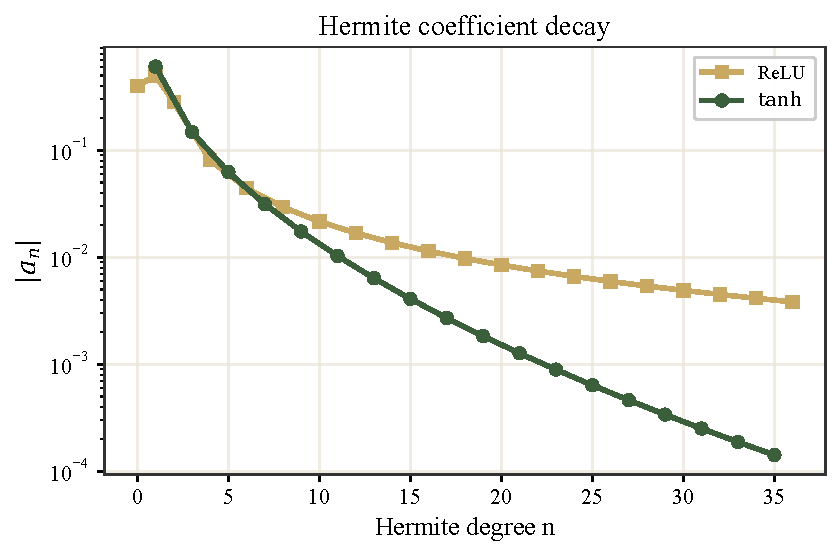
\includegraphics[width=0.7\linewidth]{figures/theory/hermite_decomposition.pdf}
    \caption{Magnitude of Hermite coefficients $|a_n|$ for \relu{} versus $\tanh$. \relu{} exhibits a slow (power-law) decay, reflecting multi-scale support across Hermite degrees, while $\tanh$ decays rapidly and concentrates most spectral mass in the lowest modes.}
    \label{fig:hermite-decomposition}
\end{figure}


\newpage










\subsection{Hermite decompositions for \relu{} and \texorpdfstring{\(\tanh\)}{tanh}}

Throughout, \(Z\sim\mathcal{N}(0,1)\) and
%
\begin{equation}
Dz \equiv \frac{dz}{\sqrt{2\pi}}e^{-z^{2}/2}.
\end{equation}
%
We expand the fixed point rescaled activation \(f(z)\) in an orthonormal Hermite basis of \(L^{2}(Dz)\),
%
\begin{equation}
f(z)=\sum_{n\ge 0} a_{n}\,h_{n}(z), \qquad a_{n}=\int Dz\,f(z)\,h_{n}(z), \qquad \int Dz\,h_{n}(z)h_{m}(z)=\delta_{nm}.
\end{equation}
%
With physicists Hermites \(H_{n}\),
%
\begin{equation}
H_{n}(x)\equiv (-1)^{n}e^{x^{2}}\frac{d^{n}}{dx^{n}}e^{-x^{2}}, \qquad h_{n}(z)\equiv \frac{1}{\sqrt{2^{n}n!}}\,H_{n}\!\left(\frac{z}{\sqrt{2}}\right).
\end{equation}
%









\subsubsection{\relu{}}

Let \(f(z)=\ReLU(z)=\max(0,z)\). The coefficients have a closed form.
%
\begin{equation}
a_{0}=\frac{1}{\sqrt{2\pi}}, \qquad a_{1}=\frac{1}{2}, \qquad a_{2k+1}=0 \ \ \text{for } k\ge 1,
\end{equation}
%
and for \(k\ge 1\),
%
\begin{equation}
a_{2k} = \frac{(-1)^{k-1}(2k-3)!!}{\sqrt{2\pi(2k)!}}.
\end{equation}
%
We use the convention \((-1)!!=1\). If instead \(f(z)=\ReLU(\sqrt{q^{*}}\,z)\), then all coefficients scale as \(a_{n}\mapsto \sqrt{q^{*}}\,a_{n}\).










\subsubsection{\texorpdfstring{\(\tanh\)}{tanh}}

Let \(f(z)=\tanh(s z)\) with \(s>0\). The coefficients are
%
\begin{equation}
a_{n}(s)=\int Dz\,\tanh(s z)\,h_{n}(z).
\end{equation}
%
Parity gives \(a_{2k}(s)=0\). There is no simple closed form for general \(s\), but the coefficients are easy to compute numerically by Gaussian quadrature using Mathematica, or other specialized packages.










\section{Experimental Details and Additional Figures}
\label{app:experimental_info}
This appendix collects the experimental details and additional figures supporting the scheduling predictions. Code for the experiments and figure generation is available at \url{https://github.com/luklacasito/dropout-mft-experiments/tree/7b8488588e4a61a0f1f6f444d7bcc8098be8406a}.










\subsection{Mean-Field Fits and Scaling Collapse}
Table~\ref{tab:mf_vs_fit_exponents} reports exponents extracted from iterated MFT recursions.
\begin{table}[ht]
\caption{Critical exponents from log--log linear fits (dashed lines) in Fig.~\ref{fig:dropout_scaling} compared with mean-field theory predictions.}
\label{tab:mf_vs_fit_exponents}
\centering
\begin{tabular}{lcc}
\toprule
Exponent & Iterated recursion & Linear approximation  \\
\midrule
$\nu$ & $1.0190 \pm 0.0014$ & $1$ \\
$\beta_{\mathrm{tanh}}$ & $0.9879 \pm 0.0007$ & $1$ \\
$\beta_{\ReLU}$ & $1.9642 \pm 0.0019$ & $2$ \\
$\theta_{\mathrm{rel,tanh}}$ & $1.0048 \pm 0.0000$ & $1$ \\
$\theta_{\mathrm{rel},\ReLU}$ & $1.9870 \pm 0.0001$ & $2$ \\
$1/\delta_{\mathrm{tanh}}$ & $0.5171 \pm 0.0007$ & $1/2$ \\
$1/\delta_{\ReLU}$ & $0.6656 \pm 0.0001$ & $2/3$ \\
$\nu_{\rho,\mathrm{tanh}}$ & $0.4716 \pm 0.0014$ & $1/2$ \\
$\nu_{\rho,\ReLU}$ & $0.3528 \pm 0.0010$ & $1/3$ \\
\bottomrule
\end{tabular}
\end{table}

The same scaling-collapse diagnostic can be carried out for the kinked universality class, using \relu{} as the representative activation. 
\begin{figure}[ht]
    \centering
    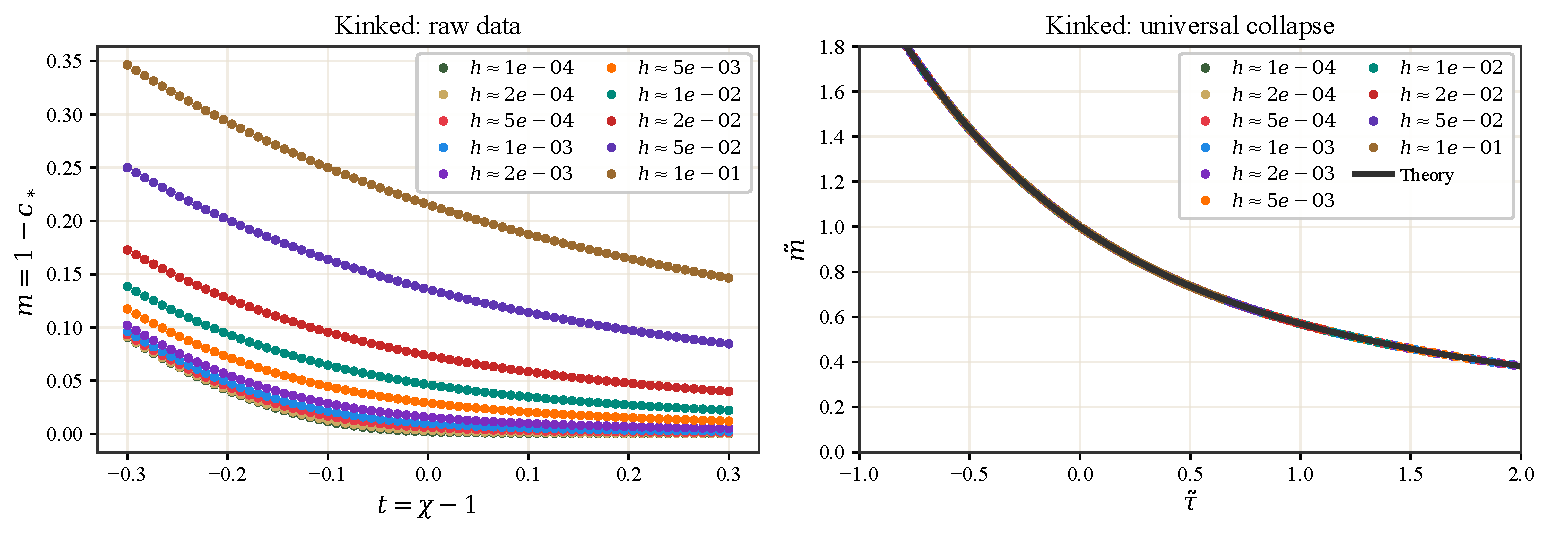
\includegraphics[width=1.0\linewidth]{figures/theory/kinked_scaling_collapse.pdf}
    \caption{Kinked counterpart to Fig.~\ref{fig:dropout_scaling}, showing the corresponding universal scaling collapse.}
    \label{fig:kinked_collapse}
\end{figure}

\FloatBarrier










\subsection{Dropout Scheduling Experiments}

The scheduling experiments below test Sec.~\ref{subsec:optimal_dropout}: MLP schedules in Fig.~\ref{fig:dropout_regimes_overfit} and Tab.~\ref{tab:dropout_summary_L6_run2}, matched-budget controls in Fig.~\ref{fig:triple_dropout} and Tab.~\ref{tab:triple_summary}, robustness sweeps in Fig.~\ref{fig:mlp_sweeps}, ViT CIFAR-100 schedules in Fig.~\ref{fig:dropout_regimes_transformer} and Tab.~\ref{tab:schedule_comparison_cifar_100}, and transformer ablations in Fig.~\ref{fig:ablations} and Tab.~\ref{tab:ablation_results}.

\FloatBarrier










\subsection{MLPs}

Finite-width experiments support these spatial scheduling predictions. The main finding is that concentrating dropout in early layers, where coadaptation and rank-diversity loss are expected to matter most, yields the best generalization. The theoretically motivated schedules improve over constant dropout at no extra computational cost.

To test this prediction in a controlled finite-width setting, we design an experiment in the overfitting regime, where information propagation and regularization are both important factors in determining performance. In the effective-theory treatment of \cite{roberts2022principlesdeeplearningtheory}, deviations from Gaussian mean-field behavior \cite{neal1996bayesian,Lee2018DNNasGP} generate corrections to the correlation recursions that are suppressed by $1/N$ (with $N$ the layer width) and accumulate across depth as $L/N$. At the same time, deep information propagation suggests that successful learning is controlled by a modest multiple of the correlation length \cite{schoenholz2017deepinformationpropagation}.

We train on 5000 CIFAR-10 images with width 256 and depth \(L=6\), roughly \(2\xi\) for the constant-dropout baseline, using a batch size of 75 to ensure the regularizing effect of dropout through injected stochastic noise. We initialize close to the edge-of-chaos at $\sigma_w^2 = 1.98$ and $\sigma_b^2 = 0.02$, near standard He initialization but avoiding the instabilities due to the divergence of the variance fixed point $q^\ast$ as $\sigma_w^2 \to 2$.

We compare six depth profiles at fixed mean dropout budget: (i) no dropout, (ii) uniform dropout, (iii) a linearly increasing schedule, (iv) a linearly decreasing schedule, (v) a step schedule concentrated in the final half (step), and (vi) a step schedule concentrated in the first half (early step), as summarized in Fig.~\ref{fig:dropout_regimes_overfit}. Front-loaded dropout consistently outperforms back-loaded dropout: the need for regularization in early layers, where coadaptation builds up most rapidly, dominates the signal propagation cost. The effective correlation length heuristic remains predictive; constant dropout is most damaging, but rank collapse breaks the permutation symmetry of Eq.~\eqref{eff_corr} in favor of early regularization.

\begin{figure*}[ht]
    \centering
    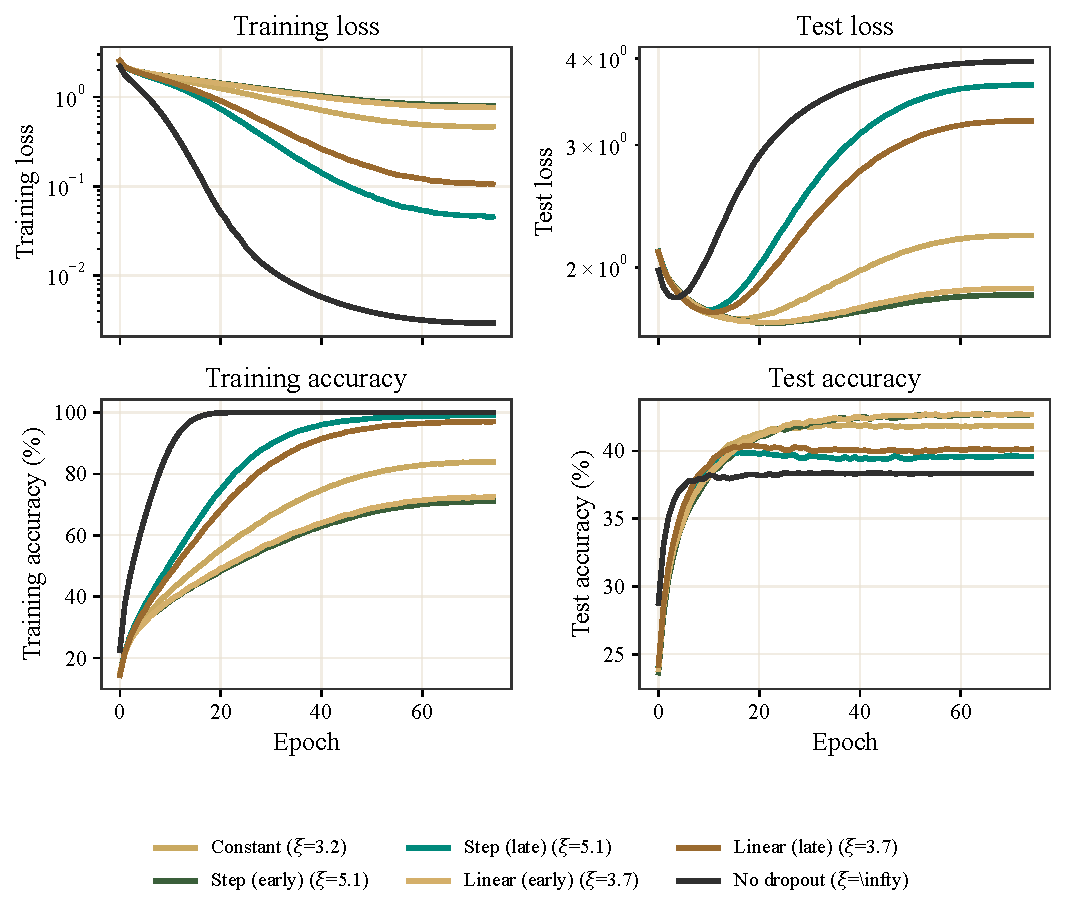
\includegraphics[width=0.8\textwidth]{figures/experiments/mlp/dropout_schedules_overfit.pdf}
    \caption{Finite-width MLP training and test curves at fixed mean dropout budget \(\bar h\) (with \(0 \le h_\ell \le h_{\max}\)). We compare uniform dropout, linear ramps (increasing/decreasing with depth), and step schedules that concentrate dropout in either
    the first or last half of the network, together with the no-dropout baseline.}
    \label{fig:dropout_regimes_overfit}
\end{figure*}


\begin{table}[t]
\caption{Performance of different dropout schedules in the overfitting regime for MLPs and CIFAR-10, corresponding to Fig.~\ref{fig:dropout_regimes_overfit}.}
\label{tab:dropout_summary_L6_run2}
\centering
\begin{tabular}{lcccc}
\hline\hline
Schedule & $\xi_{\mathrm{eff}}$ & $L/\xi_{\mathrm{eff}}$ & Best Test Acc. (\%) & Final Test Acc. (\%) \\
\hline
Constant            & $3.20$   & $1.87$ & $42.54 \pm 0.10$ & $41.84 \pm 0.10$ \\
Step (late)         & $5.09$   & $1.18$ & $40.56 \pm 0.11$ & $39.60 \pm 0.13$ \\
Step (early)        & $5.09$   & $1.18$ & $43.13 \pm 0.07$ & $42.67 \pm 0.09$ \\
Linear (increasing) & $3.73$   & $1.61$ & $41.01 \pm 0.07$ & $40.12 \pm 0.12$ \\
Linear (decreasing) & $3.73$   & $1.61$ & $43.11 \pm 0.09$ & $42.69 \pm 0.10$ \\
No dropout          & $\infty$ & $0$    & $38.77 \pm 0.10$ & $38.34 \pm 0.12$ \\
\hline\hline
\end{tabular}
\end{table}

The budget-control experiment checks a simpler explanation: early-concentrated dropout may only be winning because it raises the local dropout rate, not because the allocation over depth matters. After all, the step schedule applies dropout at rate $2\bar{h}$ to the first half of the network, so perhaps the same improvement could be achieved by applying this higher rate uniformly throughout.

To disentangle allocation from total dropout strength, we compare constant schedules with fields $\bar h,2\bar h,3\bar h$ against step schedules using $2\bar h$ in the first half or $3\bar h$ in the first third of the network (Fig.~\ref{fig:triple_dropout}, Tab.~\ref{tab:triple_summary}).
 \begin{figure}[H]
     \centering
     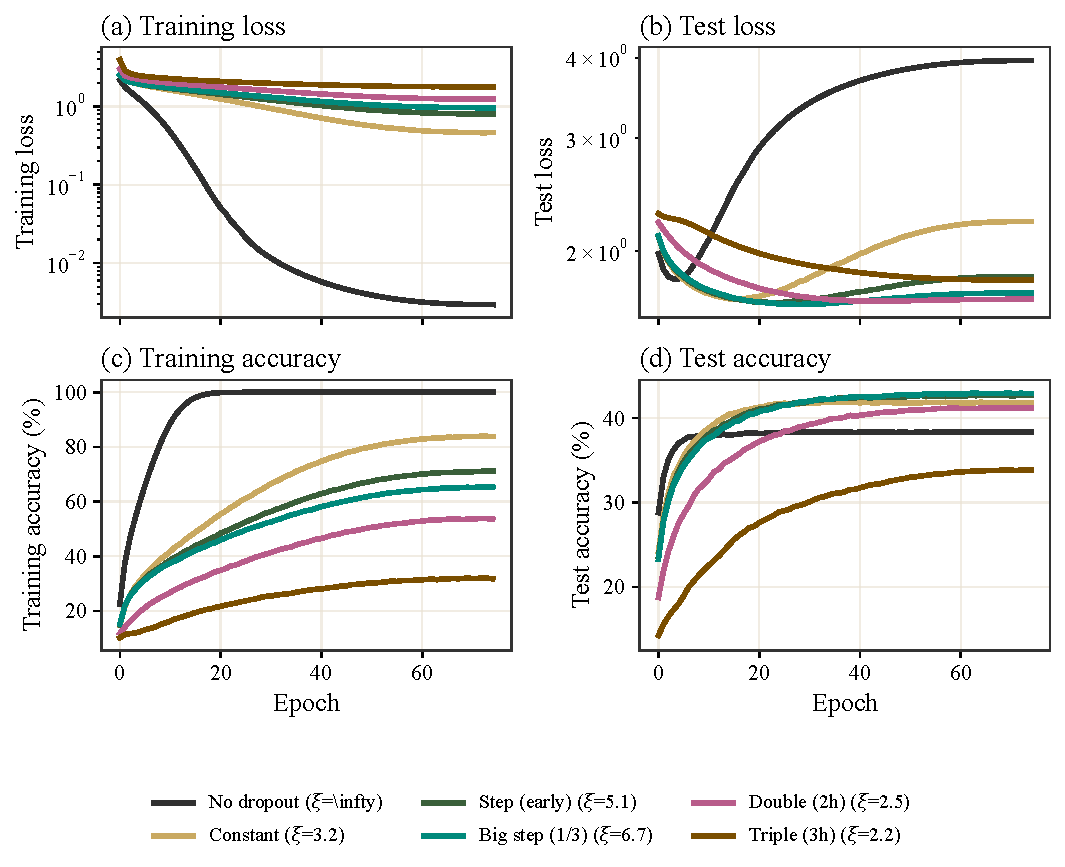
\includegraphics[width=1.0\linewidth]{figures/experiments/mlp/dropout_budget_comparison.pdf}
     \caption{Matched-budget controls comparing front-loaded step schedules against constant dropout fields at $\bar h$, $2\bar h$, and $3\bar h$.}
     \label{fig:triple_dropout}
 \end{figure}
\FloatBarrier
If the step schedules succeed merely because they apply locally higher dropout rates, then the uniform schedules with matching dropout should perform at least as well. In contrast, if spatial allocation genuinely matters, the step schedules should outperform their uniform counterparts despite having lower total dropout.
The results in Fig.~\ref{fig:triple_dropout} and Table~\ref{tab:triple_summary} confirm that spatial allocation dominates: Big step ($\xi_{\text{eff}} = 6.7$) achieves the highest accuracy despite having only one-third the total dropout of the schedule with $3\bar h$, and front-loaded step ($\xi_{\text{eff}} = 5.1$) outperforms Double despite half the total dropout budget. Moreover, increasing uniform dropout beyond $2\bar{h}$ becomes counterproductive; Triple ($3\bar{h}$) performs worst among all dropout schedules, as excessive regularization throughout the network impairs learning capacity. These findings validate the effective correlation length $\xi_{\text{eff}}$ as a predictive metric: schedules with longer $\xi_{\text{eff}}$ consistently achieve better generalization, regardless of their total dropout budget.

We note that our theoretical analysis is perturbative in $h$, with higher-order corrections of $O(h^2)$ becoming significant as dropout increases. This motivates our choice to test up to $3\bar{h}$ with $\bar h=0.1$; beyond this point, the perturbative framework becomes less reliable and additional nonlinear effects may dominate. We also tested these effects at lower dropout rates and obtained similar results, though they become more pronounced as dropout increases. 




\begin{table}[ht]
\caption{Summary of dropout schedules, correlation lengths, and test performance for MLPs on CIFAR-10, corresponding to Fig.~\ref{fig:triple_dropout}.}
\label{tab:triple_summary}
\centering
\begin{tabular}{lcccc}
\hline\hline
Schedule & $\xi_{\mathrm{eff}}$ & $L/\xi_{\mathrm{eff}}$ & Best Test Acc. (\%) & Final Test Acc. (\%) \\
\hline
No dropout          & $\infty$ & $0.00$ & $38.77 \pm 0.10$ & $38.34 \pm 0.12$ \\
Constant            & $3.20$   & $1.87$ & $42.54 \pm 0.10$ & $41.84 \pm 0.10$ \\
Step (early)        & $5.09$   & $1.18$ & $43.13 \pm 0.07$ & $42.67 \pm 0.09$ \\
Big step (1/3)      & $6.67$   & $0.90$ & $43.29 \pm 0.08$ & $42.92 \pm 0.10$ \\
Double ($2\bar{h}$) & $2.54$   & $2.36$ & $41.46 \pm 0.08$ & $41.19 \pm 0.10$ \\
Triple ($3\bar{h}$) & $2.22$   & $2.70$ & $33.94 \pm 0.22$ & $33.82 \pm 0.23$ \\
\hline\hline
\end{tabular}
\end{table}


\begin{table}[h]
    \caption{Experimental and hyperparameter configuration for high overfitting regime. Corresponding performance metrics in Fig.~\ref{fig:dropout_regimes_overfit}.}
    \label{tab:experiment_config_2}
    \centering
    \begin{tabular}{l l}
        \toprule
        \textbf{Parameter} & \textbf{Value / Description} \\
        \midrule
        \multicolumn{2}{l}{\textit{Network Architecture \& Initialization}} \\
        \midrule
        Network Width & 256 \\
        Depth Multiplier & 2 \\
        Weight Variance ($\sigma_w^2$) & 1.98 \\
        Bias Variance ($\sigma_b^2$) & 0.02 \\
        
        \midrule
        \multicolumn{2}{l}{\textit{Training Dynamics}} \\
        \midrule
        Epochs & 50 \\
        Batch Size & 75 \\
        Learning Rate & $1 \times 10^{-4}$ \\
        LR Schedule & Decay to minimum $1 \times 10^{-7}$ \\
        Mean Dropout Field ($\bar{h}$) & 0.1 \\
        Max Dropout Field ($h_{\max}$) & 0.2 (Step); 0.3 (Big step) \\
        Step Active Fraction ($f$) & $1/2$ (Step); $1/3$ (Big step) \\
        \midrule
        \multicolumn{2}{l}{\textit{General Setup}} \\
        \midrule
        Number of Simulations & 20 \\
        Dataset Usage & CIFAR-10 5,000 samples \\
        Hardware & GPU A100  \\
        \bottomrule
    \end{tabular}
\end{table}

\FloatBarrier










\subsection{Robustness Sweeps}
\label{app:sweeps}
\setlength{\textfloatsep}{6pt plus 1pt minus 2pt}
\setlength{\floatsep}{6pt plus 1pt minus 2pt}
\setlength{\dbltextfloatsep}{6pt plus 1pt minus 2pt}
\setlength{\dblfloatsep}{6pt plus 1pt minus 2pt}

To test whether scheduling is tied to one budget, width, or activation, we ran CIFAR-10 MLP sweeps (Figs.~\ref{fig:mlp_sweeps} and \ref{fig:gelu_h_sweep}). The \relu{} sweeps probe mean-field boundaries: at \(\bar h=0.15\), Step/Big step use nonperturbative local fields \(0.30/0.45\); at \(N=64\), finite-width non-Gaussianity weakens the correlation-length prediction. The GELU MLP sweep gives the same best-accuracy ordering at \(\bar h=0.1\)--constant \(41.96\pm0.16\), Step \(42.24\pm0.15\), Big step \(42.46\pm0.12\)--and Big step falls to \(38.97\pm0.23\) at \(\bar h=0.15\), matching this perturbative-boundary picture. The final-epoch gains summarized in Table~\ref{tab:loss_improvements} use the last recorded epoch, giving \(+2.04\) pp for the \relu{} \(\bar h=0.1\) sweep and \(+0.62\) pp for the GELU \(\bar h=0.1\) sweep.

\begin{figure*}[t]
    \centering
    \subfigure[Sweep over mean dropout field at width \(N=256\).]{
        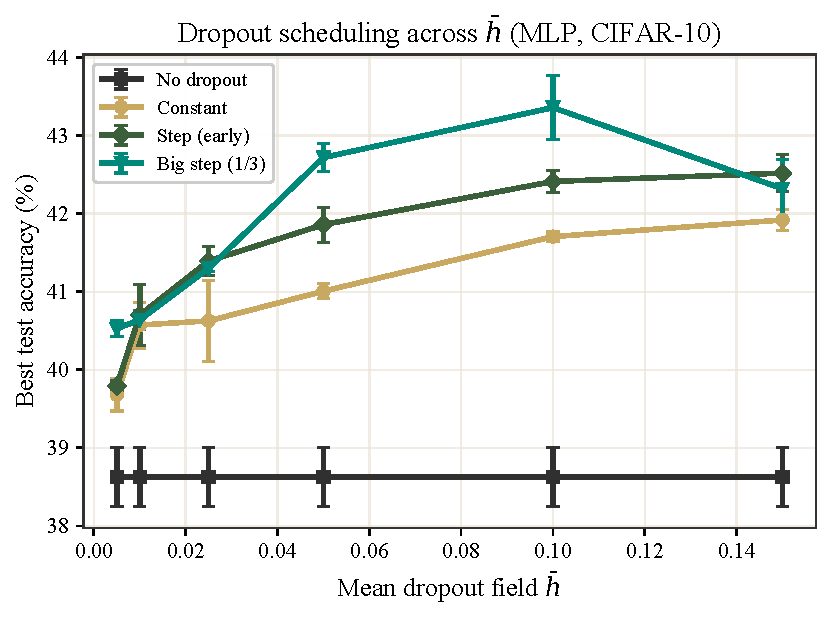
\includegraphics[width=0.45\textwidth]{figures/experiments/sweeps/h_sweep_schedule_comparison.pdf}
    }
    \subfigure[Schedule advantage over constant dropout at \(\bar h=0.1\).]{
        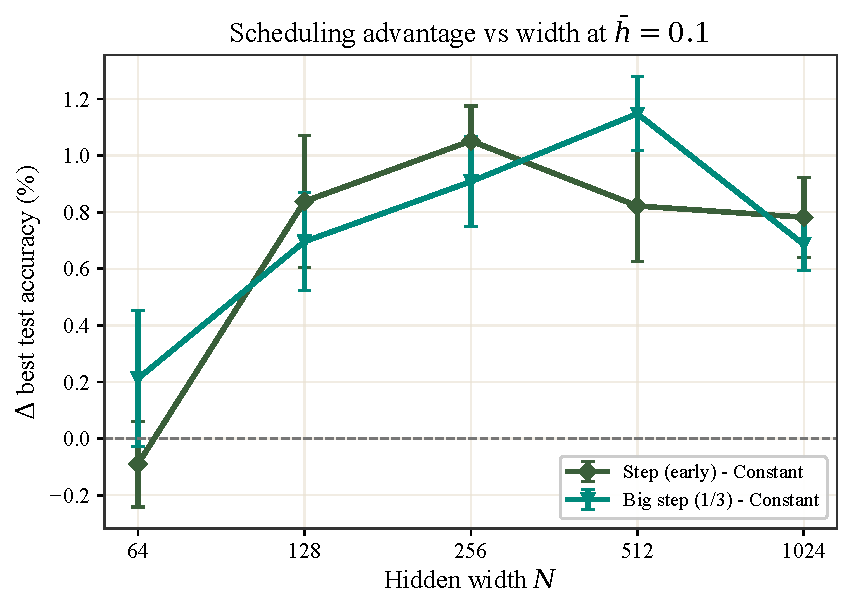
\includegraphics[width=0.45\textwidth]{figures/experiments/sweeps/width_sweep_baseline_advantage.pdf}
    }
    \caption{Robustness sweeps for depth-6 near-critical \relu{} MLPs on CIFAR-10. Early schedules improve over constant dropout throughout the large-width regime, while \(N=64\) illustrates the expected finite-width boundary.}
    \label{fig:mlp_sweeps}
\end{figure*}

\begin{figure*}[t]
    \centering
    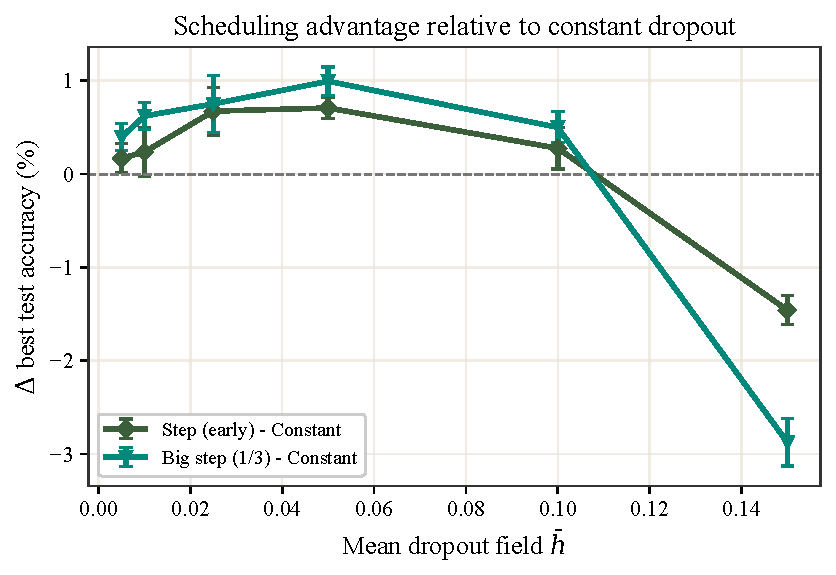
\includegraphics[width=0.72\textwidth]{figures/experiments/sweeps/gelu_h_sweep_delta.pdf}
    \caption{Smooth-activation \(h\)-sweep for depth-6 near-critical GELU MLPs on CIFAR-10 at width \(N=256\). Step-like schedules improve over constant dropout around \(\bar h=0.1\), while the largest field leaves the small-dropout regime where the mean-field perturbation is expected to be predictive.}
    \label{fig:gelu_h_sweep}
\end{figure*}

\FloatBarrier










\subsection{Transformers on CIFAR-100}
Table~\ref{tab:vit_config} and Fig.~\ref{fig:dropout_regimes_transformer} detail the architectural parameters and corresponding test dynamics for the CIFAR-100 Vision Transformer evaluation \cite{dosovitskiy2021vit,krizhevsky2009cifar}; Table~\ref{tab:schedule_comparison_cifar_100} reports the schedule comparison. 
\begin{figure*}[h]
    \centering
    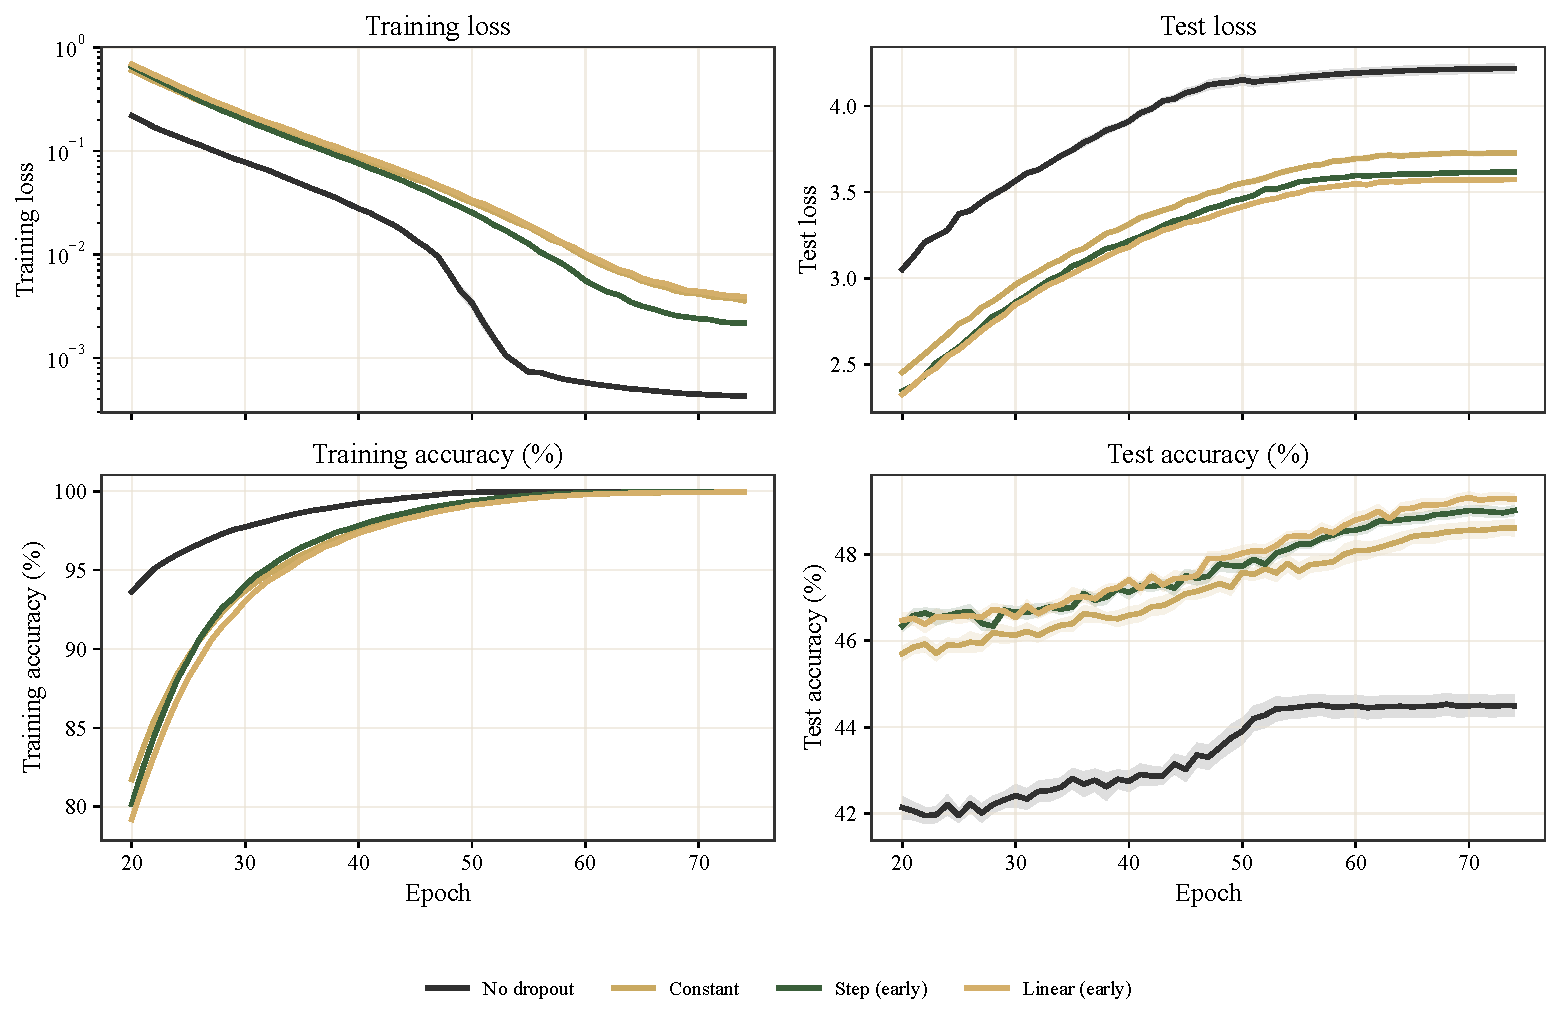
\includegraphics[width=0.95\textwidth]{figures/experiments/transformer/dropout_schedules_cropped.pdf}
    \caption{Finite-width Vision Transformer training and test curves at fixed mean dropout budget \(\bar h\). We compare the no-dropout baseline, uniform dropout, decreasing linear ramps, and early step schedules. The cropped view shows epochs 20--75 for readability; the full curve is also in App.~\ref{app:experimental_info}.}
    \label{fig:dropout_regimes_transformer}
\end{figure*}
\begin{figure}[t]
    \centering
    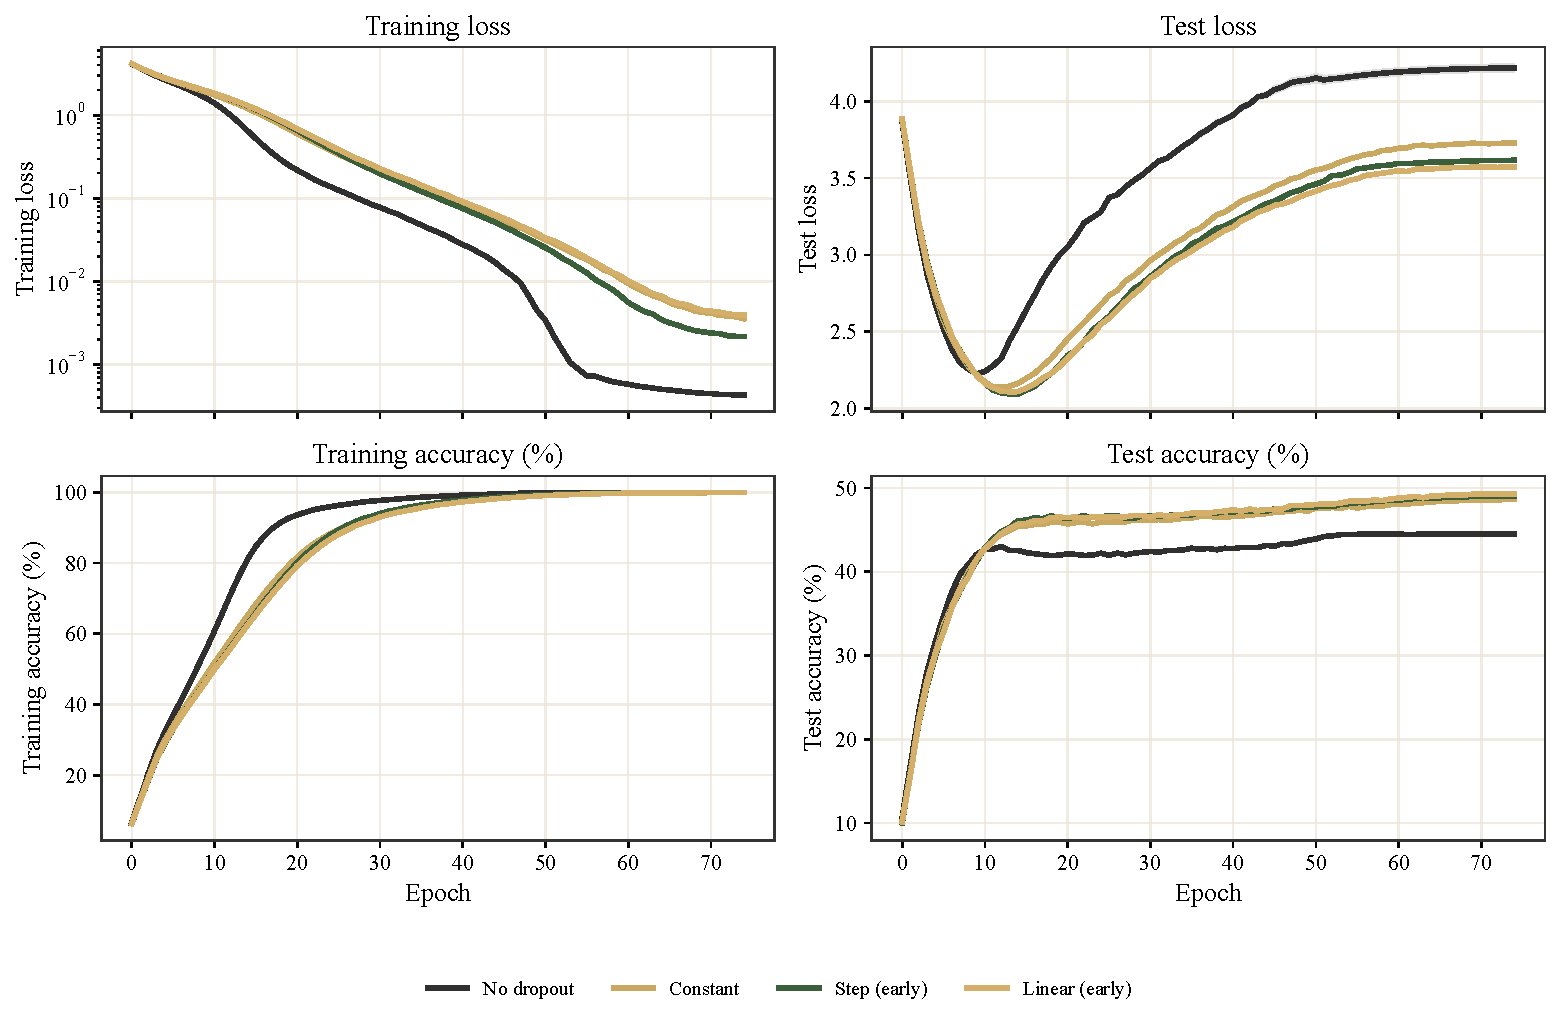
\includegraphics[width=0.95\linewidth]{figures/experiments/transformer/dropout_schedules_full.pdf}
    \caption{Extended training curves for Figure~\ref{fig:dropout_regimes_transformer}, showing the full 75 epochs.}
    \label{fig:transformer_full}
\end{figure}

\begin{table}[h]
    \caption{Experimental configuration for Vision Transformer (ViT) simulations.}
    \label{tab:vit_config}
    \centering
    \footnotesize
    \setlength{\tabcolsep}{3pt}
    \renewcommand{\arraystretch}{0.9}
    \begin{tabular}{l l}
        \toprule
        \textbf{Parameter} & \textbf{Value / Description} \\
        \midrule
        \multicolumn{2}{l}{\textit{ViT Architecture}} \\
        \midrule
        Embedding Dimension & 128 \\
        Depth & 12 \\
        Number of Heads & 16 \\
        MLP Ratio & 4.0 \\
        Patch Size & 4 \\
        \midrule
        \multicolumn{2}{l}{\textit{Training Dynamics}} \\
        \midrule
        Epochs & 75 \\
        Batch Size & 250 \\
        Learning Rate & $5 \times 10^{-4}$ \\
        LR Minimum & $5 \times 10^{-6}$ \\
        Weight Decay & 0.00 \\
        Mean Dropout Field ($\bar{h}$) & 0.1 \\
        Max Dropout Field ($h_{\max}$) & 0.2 \\
        Schedules & None, Constant, Step (early), Linear (decreasing) \\
        \midrule
        \multicolumn{2}{l}{\textit{General Setup}} \\
        \midrule
        Number of Simulations & 10 \\
        Dataset Usage & Full CIFAR-100 \\
        Evaluation Frequency & Every 1 Epoch \\
        Hardware & GPU A100  \\
        \bottomrule
    \end{tabular}
\end{table}

Accuracy curves are shown in Fig.~\ref{fig:dropout_regimes_transformer}, with explicit results in Table~\ref{tab:schedule_comparison_cifar_100}. All reported errors are SEM. On CIFAR-100 (and similarly on CIFAR-10), concentrating dropout earlier consistently improved accuracy and reduced overfitting. Interestingly, linear decreasing schedules, which put more dropout in early layers, often performed especially well in transformers; residual connections were introduced in \cite{he2016resnet}, and mean-field analyses show that they ease information propagation \cite{yang2017meanfieldresnets}. We suspect this makes distributing regularization early preferable empirically, though both early weighted and step-like schedules outperformed the constant baseline.

We focus on controlled regimes rather than ImageNet-scale benchmarking because our central claims are mechanistic and derived in a mean-field initialization framework, which is most cleanly tested when finite-width corrections remain subdominant. The experimental validation is designed to test the theory in settings where MFT predictions apply cleanly, rather than to establish state-of-the-art performance on large-scale datasets such as ImageNet \cite{imagenet}. ImageNet-scale training introduces substantial confounders from augmentation and extensive hyperparameter tuning that can obscure MFT effects; we leave that evaluation as future work. In these controlled runs, the predicted schedules outperform constant dropout, illustrating the practical utility of the mean-field framework.

\begin{table}[h]
    \caption{Test accuracy across different dropout schedules for ViT architecture on CIFAR-100, corresponding to Fig.~\ref{fig:dropout_regimes_transformer}.}
    \label{tab:schedule_comparison_cifar_100}
    \centering
    \footnotesize
    \begin{tabular}{l c c}
    \toprule
    \textbf{Schedule} & \textbf{Best Test Acc} & \textbf{Final Test Acc} \\
    \midrule
    No dropout          & $44.61 \pm 0.25$ & $44.50 \pm 0.25$ \\
    Constant            & $48.69 \pm 0.18$ & $48.61 \pm 0.20$ \\
    Step (early)        & $49.10 \pm 0.11$ & $49.01 \pm 0.12$ \\
    Linear (decreasing) & $49.38 \pm 0.14$ & $49.27 \pm 0.14$ \\
    \bottomrule
    \end{tabular}
\end{table}

\FloatBarrier
\clearpage










\subsection{Transformer Ablations}
To isolate the effect of dropout scheduling on distinct transformer components, we performed component-level ablations. We tested transformers with dropout applied exclusively to the attention block, the MLP block, or both, comparing step-like and constant schedules against a no-dropout baseline. Experimental hyperparameters are listed in Table~\ref{tab:ablation_config}; they largely mirror the main transformer experiment, though we conducted five simulations per configuration. Additionally, we tested these theoretical results on a second dataset, CIFAR-10.

\begin{figure}[H]
    \centering
    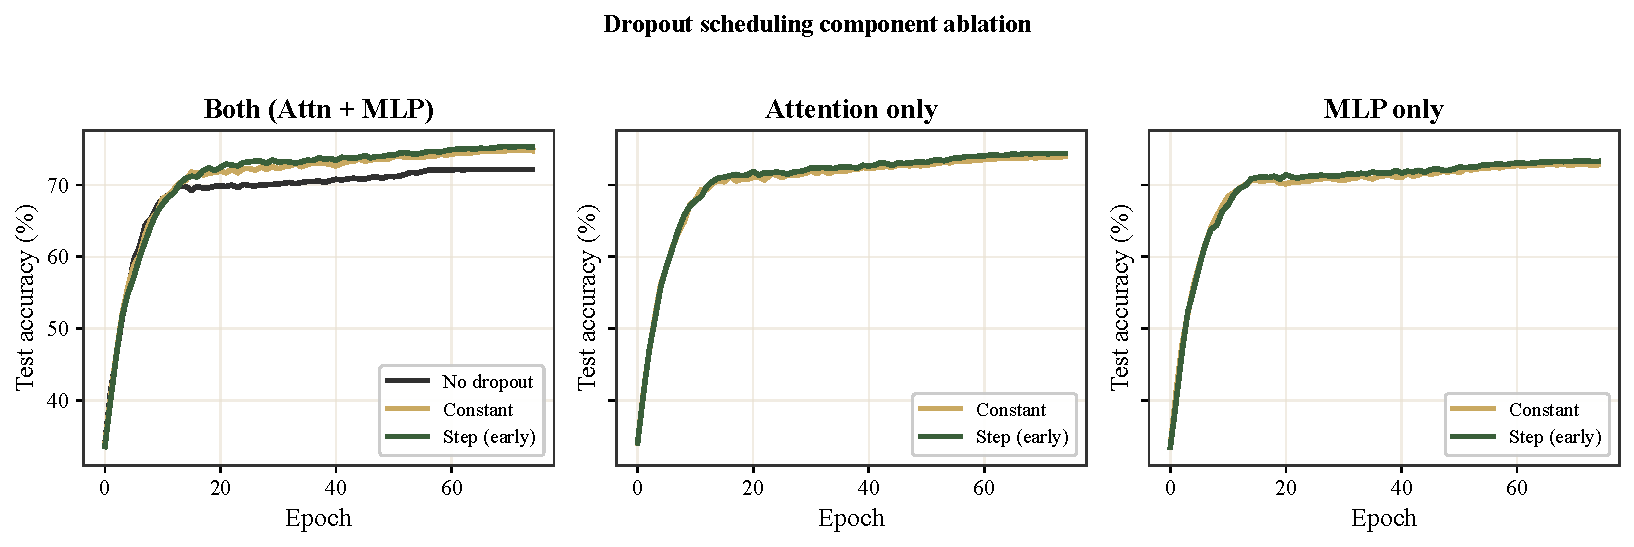
\includegraphics[width=1\linewidth]{figures/experiments/transformer/component_ablations.pdf}
    \caption{Component ablations applying dropout schedules to the attention block, MLP block, or both. The figure compares no dropout, constant dropout, and step-like dropout.}
    \label{fig:ablations}
\end{figure}

\begin{table}[h]
    \caption{Experimental configuration for Vision Transformer (ViT) ablation study.}
    \label{tab:ablation_config}
    \centering
    \footnotesize
    \setlength{\tabcolsep}{3pt}
    \renewcommand{\arraystretch}{0.9}
    \begin{tabular}{l l}
        \toprule
        \textbf{Parameter} & \textbf{Value / Description} \\
        \midrule
        \multicolumn{2}{l}{\textit{ViT Architecture}} \\
        \midrule
        Embedding Dimension & 128 \\
        Depth & 12 \\
        Number of Heads & 16 \\
        MLP Ratio & 4.0 \\
        Patch Size & 4 \\
        \midrule
        \multicolumn{2}{l}{\textit{Training Dynamics}} \\
        \midrule
        Epochs & 75 \\
        Batch Size & 1000 \\
        Learning Rate & $5 \times 10^{-4}$ \\
        LR Minimum & $5 \times 10^{-6}$ \\
        Weight Decay & 0.00 \\
        Mean Dropout Field ($\bar{h}$) & 0.1 \\
        Max Dropout Field ($h_{\max}$) & 0.2 \\
        Schedules & None, Constant, Step (early) \\
        Ablation Modes & Both, Attention-only, MLP-only \\
        \midrule
        \multicolumn{2}{l}{\textit{General Setup}} \\
        \midrule
        Number of Simulations & 5 \\
        Dataset Usage & Full CIFAR-10 \\
        Evaluation Frequency & Every 1 Epoch \\
        Hardware & GPU A100\\
        \bottomrule
    \end{tabular}
\end{table}

\begin{table}[H]
    \caption{Component-level ablations on CIFAR-10, comparing Constant and Step-like dropout schedules applied exclusively to the MLP block, Attention block, or both. The Step (early) schedule consistently outperforms the Constant schedule across all configurations.}
    \label{tab:ablation_results}
    \centering
    \begin{tabular}{l c c}
        \toprule
        \textbf{Configuration} & \textbf{Best Test Acc} & \textbf{Final Test Acc} \\
        \midrule
        No dropout & $72.22 \pm 0.31$ & $72.15 \pm 0.33$ \\
        \midrule
        MLP only (Constant) & $72.96 \pm 0.26$ & $72.88 \pm 0.28$ \\
        MLP only (Step early) & $73.38 \pm 0.56$ & $73.29 \pm 0.55$ \\
        \midrule
        Attn only (Constant) & $74.00 \pm 0.20$ & $73.95 \pm 0.21$ \\
        Attn only (Step early) & $74.48 \pm 0.20$ & $74.41 \pm 0.19$ \\
        \midrule
        Both (Constant) & $74.92 \pm 0.22$ & $74.78 \pm 0.23$ \\
        Both (Step early) & $75.47 \pm 0.27$ & $75.30 \pm 0.29$ \\
        \bottomrule
    \end{tabular}
\end{table}

\FloatBarrier

\end{document}



% This document was modified from the file originally made available by
% Pat Langley and Andrea Danyluk for ICML-2K. This version was created
% by Iain Murray in 2018, and modified by Alexandre Bouchard in
% 2019 and 2021 and by Csaba Szepesvari, Gang Niu and Sivan Sabato in 2022.
% Modified again in 2023 and 2024 by Sivan Sabato and Jonathan Scarlett.
% Previous contributors include Dan Roy, Lise Getoor and Tobias
% Scheffer, which was slightly modified from the 2010 version by
% Thorsten Joachims & Johannes Fuernkranz, slightly modified from the
% 2009 version by Kiri Wagstaff and Sam Roweis's 2008 version, which is
% slightly modified from Prasad Tadepalli's 2007 version which is a
% lightly changed version of the previous year's version by Andrew
% Moore, which was in turn edited from those of Kristian Kersting and
% Codrina Lauth. Alex Smola contributed to the algorithmic style files.
